\documentclass[1p]{elsarticle_modified}
%\bibliographystyle{elsarticle-num}

%\usepackage[colorlinks]{hyperref}
%\usepackage{abbrmath_seonhwa} %\Abb, \Ascr, \Acal ,\Abf, \Afrak
\usepackage{amsfonts}
\usepackage{amssymb}
\usepackage{amsmath}
\usepackage{amsthm}
\usepackage{scalefnt}
\usepackage{amsbsy}
\usepackage{kotex}
\usepackage{caption}
\usepackage{subfig}
\usepackage{color}
\usepackage{graphicx}
\usepackage{xcolor} %% white, black, red, green, blue, cyan, magenta, yellow
\usepackage{float}
\usepackage{setspace}
\usepackage{hyperref}

\usepackage{tikz}
\usetikzlibrary{arrows}

\usepackage{multirow}
\usepackage{array} % fixed length table
\usepackage{hhline}

%%%%%%%%%%%%%%%%%%%%%
\makeatletter
\renewcommand*\env@matrix[1][\arraystretch]{%
	\edef\arraystretch{#1}%
	\hskip -\arraycolsep
	\let\@ifnextchar\new@ifnextchar
	\array{*\c@MaxMatrixCols c}}
\makeatother %https://tex.stackexchange.com/questions/14071/how-can-i-increase-the-line-spacing-in-a-matrix
%%%%%%%%%%%%%%%

\usepackage[normalem]{ulem}

\newcommand{\msout}[1]{\ifmmode\text{\sout{\ensuremath{#1}}}\else\sout{#1}\fi}
%SOURCE: \msout is \stkout macro in https://tex.stackexchange.com/questions/20609/strikeout-in-math-mode

\newcommand{\cancel}[1]{
	\ifmmode
	{\color{red}\msout{#1}}
	\else
	{\color{red}\sout{#1}}
	\fi
}

\newcommand{\add}[1]{
	{\color{blue}\uwave{#1}}
}

\newcommand{\replace}[2]{
	\ifmmode
	{\color{red}\msout{#1}}{\color{blue}\uwave{#2}}
	\else
	{\color{red}\sout{#1}}{\color{blue}\uwave{#2}}
	\fi
}

\newcommand{\Sol}{\mathcal{S}} %segment
\newcommand{\D}{D} %diagram
\newcommand{\A}{\mathcal{A}} %arc


%%%%%%%%%%%%%%%%%%%%%%%%%%%%%5 test

\def\sl{\operatorname{\textup{SL}}(2,\Cbb)}
\def\psl{\operatorname{\textup{PSL}}(2,\Cbb)}
\def\quan{\mkern 1mu \triangleright \mkern 1mu}

\theoremstyle{definition}
\newtheorem{thm}{Theorem}[section]
\newtheorem{prop}[thm]{Proposition}
\newtheorem{lem}[thm]{Lemma}
\newtheorem{ques}[thm]{Question}
\newtheorem{cor}[thm]{Corollary}
\newtheorem{defn}[thm]{Definition}
\newtheorem{exam}[thm]{Example}
\newtheorem{rmk}[thm]{Remark}
\newtheorem{alg}[thm]{Algorithm}

\newcommand{\I}{\sqrt{-1}}
\begin{document}

%\begin{frontmatter}
%
%\title{Boundary parabolic representations of knots up to 8 crossings}
%
%%% Group authors per affiliation:
%\author{Yunhi Cho} 
%\address{Department of Mathematics, University of Seoul, Seoul, Korea}
%\ead{yhcho@uos.ac.kr}
%
%
%\author{Seonhwa Kim} %\fnref{s_kim}}
%\address{Center for Geometry and Physics, Institute for Basic Science, Pohang, 37673, Korea}
%\ead{ryeona17@ibs.re.kr}
%
%\author{Hyuk Kim}
%\address{Department of Mathematical Sciences, Seoul National University, Seoul 08826, Korea}
%\ead{hyukkim@snu.ac.kr}
%
%\author{Seokbeom Yoon}
%\address{Department of Mathematical Sciences, Seoul National University, Seoul, 08826,  Korea}
%\ead{sbyoon15@snu.ac.kr}
%
%\begin{abstract}
%We find all boundary parabolic representation of knots up to 8 crossings.
%
%\end{abstract}
%\begin{keyword}
%    \MSC[2010] 57M25 
%\end{keyword}
%
%\end{frontmatter}

%\linenumbers
%\tableofcontents
%
\newcommand\colored[1]{\textcolor{white}{\rule[-0.35ex]{0.8em}{1.4ex}}\kern-0.8em\color{red} #1}%
%\newcommand\colored[1]{\textcolor{white}{ #1}\kern-2.17ex	\textcolor{white}{ #1}\kern-1.81ex	\textcolor{white}{ #1}\kern-2.15ex\color{red}#1	}

{\Large $\underline{12a_{1004}~(K12a_{1004})}$}

\setlength{\tabcolsep}{10pt}
\renewcommand{\arraystretch}{1.6}
\vspace{1cm}\begin{tabular}{m{100pt}>{\centering\arraybackslash}m{274pt}}
\multirow{5}{120pt}{
	\centering
	\includegraphics[width=112pt]{../../../GIT/diagram.site/Diagrams/png/1805_12a_1004.png}\\
\ \ \ A knot diagram\footnotemark}&
\allowdisplaybreaks
\textbf{Linearized knot diagam} \\
\cline{2-2}
 &
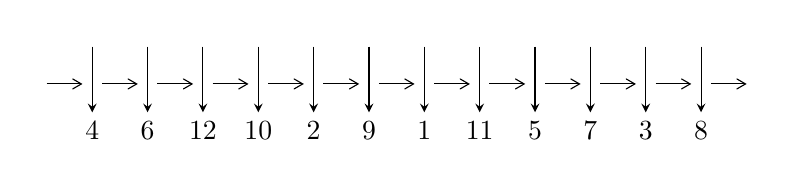
\begin{tikzpicture}[x=20pt, y=17pt]
	% nodes
	\node (C0) at (0, 0) {};
	\node (C1) at (1, 0) {};
	\node (C1U) at (1, +1) {};
	\node (C1D) at (1, -1) {4};

	\node (C2) at (2, 0) {};
	\node (C2U) at (2, +1) {};
	\node (C2D) at (2, -1) {6};

	\node (C3) at (3, 0) {};
	\node (C3U) at (3, +1) {};
	\node (C3D) at (3, -1) {12};

	\node (C4) at (4, 0) {};
	\node (C4U) at (4, +1) {};
	\node (C4D) at (4, -1) {10};

	\node (C5) at (5, 0) {};
	\node (C5U) at (5, +1) {};
	\node (C5D) at (5, -1) {2};

	\node (C6) at (6, 0) {};
	\node (C6U) at (6, +1) {};
	\node (C6D) at (6, -1) {9};

	\node (C7) at (7, 0) {};
	\node (C7U) at (7, +1) {};
	\node (C7D) at (7, -1) {1};

	\node (C8) at (8, 0) {};
	\node (C8U) at (8, +1) {};
	\node (C8D) at (8, -1) {11};

	\node (C9) at (9, 0) {};
	\node (C9U) at (9, +1) {};
	\node (C9D) at (9, -1) {5};

	\node (C10) at (10, 0) {};
	\node (C10U) at (10, +1) {};
	\node (C10D) at (10, -1) {7};

	\node (C11) at (11, 0) {};
	\node (C11U) at (11, +1) {};
	\node (C11D) at (11, -1) {3};

	\node (C12) at (12, 0) {};
	\node (C12U) at (12, +1) {};
	\node (C12D) at (12, -1) {8};
	\node (C13) at (13, 0) {};

	% arrows
	\draw[->,>={angle 60}]
	(C0) edge (C1) (C1) edge (C2) (C2) edge (C3) (C3) edge (C4) (C4) edge (C5) (C5) edge (C6) (C6) edge (C7) (C7) edge (C8) (C8) edge (C9) (C9) edge (C10) (C10) edge (C11) (C11) edge (C12) (C12) edge (C13) ;	\draw[->,>=stealth]
	(C1U) edge (C1D) (C2U) edge (C2D) (C3U) edge (C3D) (C4U) edge (C4D) (C5U) edge (C5D) (C6U) edge (C6D) (C7U) edge (C7D) (C8U) edge (C8D) (C9U) edge (C9D) (C10U) edge (C10D) (C11U) edge (C11D) (C12U) edge (C12D) ;
	\end{tikzpicture} \\
\hhline{~~} \\& 
\textbf{Solving Sequence} \\ \cline{2-2} 
 &
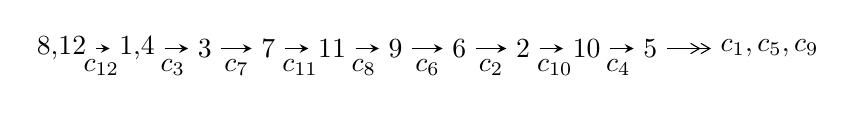
\begin{tikzpicture}[x=23pt, y=7pt]
	% node
	\node (A0) at (-1/8, 0) {8,12};
	\node (A1) at (17/16, 0) {1,4};
	\node (A2) at (17/8, 0) {3};
	\node (A3) at (25/8, 0) {7};
	\node (A4) at (33/8, 0) {11};
	\node (A5) at (41/8, 0) {9};
	\node (A6) at (49/8, 0) {6};
	\node (A7) at (57/8, 0) {2};
	\node (A8) at (65/8, 0) {10};
	\node (A9) at (73/8, 0) {5};
	\node (C1) at (1/2, -1) {$c_{12}$};
	\node (C2) at (13/8, -1) {$c_{3}$};
	\node (C3) at (21/8, -1) {$c_{7}$};
	\node (C4) at (29/8, -1) {$c_{11}$};
	\node (C5) at (37/8, -1) {$c_{8}$};
	\node (C6) at (45/8, -1) {$c_{6}$};
	\node (C7) at (53/8, -1) {$c_{2}$};
	\node (C8) at (61/8, -1) {$c_{10}$};
	\node (C9) at (69/8, -1) {$c_{4}$};
	\node (A10) at (11, 0) {$c_{1},c_{5},c_{9}$};

	% edge
	\draw[->,>=stealth]	
	(A0) edge (A1) (A1) edge (A2) (A2) edge (A3) (A3) edge (A4) (A4) edge (A5) (A5) edge (A6) (A6) edge (A7) (A7) edge (A8) (A8) edge (A9) ;
	\draw[->>,>={angle 60}]	
	(A9) edge (A10);
\end{tikzpicture} \\ 

\end{tabular} \\

\footnotetext{
The image of knot diagram is generated by the software ``\textbf{Draw programme}" developed by Andrew Bartholomew(\url{http://www.layer8.co.uk/maths/draw/index.htm\#Running-draw}), where we modified some parts for our purpose(\url{https://github.com/CATsTAILs/LinksPainter}).
}\phantom \\ \newline 
\centering \textbf{Ideals for irreducible components\footnotemark of $X_{\text{par}}$} 
 
\begin{align*}
I^u_{1}&=\langle 
2.50144\times10^{15} u^{30}+1.24069\times10^{15} u^{29}+\cdots+2.15585\times10^{16} b+1.38288\times10^{16},\\
\phantom{I^u_{1}}&\phantom{= \langle  }-5.21559\times10^{15} u^{30}+7.73030\times10^{12} u^{29}+\cdots+2.15585\times10^{16} a-2.45094\times10^{16},\\
\phantom{I^u_{1}}&\phantom{= \langle  }u^{31}+11 u^{29}+\cdots+12 u+4\rangle \\
I^u_{2}&=\langle 
1.75494\times10^{735} u^{149}+8.27613\times10^{735} u^{148}+\cdots+4.56524\times10^{736} b+8.92522\times10^{738},\\
\phantom{I^u_{2}}&\phantom{= \langle  }-1.97153\times10^{738} u^{149}-3.62879\times10^{738} u^{148}+\cdots+1.39848\times10^{739} a-5.96878\times10^{740},\\
\phantom{I^u_{2}}&\phantom{= \langle  }u^{150}+2 u^{149}+\cdots-2018 u+919\rangle \\
I^u_{3}&=\langle 
u^5+u^4+2 u^3+u^2+2 b+u-1,\;- u^5- u^4-2 u^3+u^2+2 a- u+3,\;u^6+3 u^4- u^3+2 u^2-2 u-1\rangle \\
I^u_{4}&=\langle 
4.40374\times10^{51} u^{45}-8.43737\times10^{51} u^{44}+\cdots+5.41181\times10^{50} b-4.27132\times10^{52},\\
\phantom{I^u_{4}}&\phantom{= \langle  }-3.42335\times10^{52} u^{45}+1.28492\times10^{52} u^{44}+\cdots+1.08236\times10^{51} a-1.08479\times10^{53},\;u^{46}- u^{45}+\cdots+12 u+4\rangle \\
\\
\end{align*}
\raggedright * 4 irreducible components of $\dim_{\mathbb{C}}=0$, with total 233 representations.\\
\footnotetext{All coefficients of polynomials are rational numbers. But the coefficients are sometimes approximated in decimal forms when there is not enough margin.}
\newpage
\renewcommand{\arraystretch}{1}
\centering \section*{I. $I^u_{1}= \langle 2.50\times10^{15} u^{30}+1.24\times10^{15} u^{29}+\cdots+2.16\times10^{16} b+1.38\times10^{16},\;-5.22\times10^{15} u^{30}+7.73\times10^{12} u^{29}+\cdots+2.16\times10^{16} a-2.45\times10^{16},\;u^{31}+11 u^{29}+\cdots+12 u+4 \rangle$}
\flushleft \textbf{(i) Arc colorings}\\
\begin{tabular}{m{7pt} m{180pt} m{7pt} m{180pt} }
\flushright $a_{8}=$&$\begin{pmatrix}0\\u\end{pmatrix}$ \\
\flushright $a_{12}=$&$\begin{pmatrix}1\\0\end{pmatrix}$ \\
\flushright $a_{1}=$&$\begin{pmatrix}1\\u^2\end{pmatrix}$ \\
\flushright $a_{4}=$&$\begin{pmatrix}0.241927 u^{30}-0.000358573 u^{29}+\cdots+1.43030 u+1.13688\\-0.116030 u^{30}-0.0575497 u^{29}+\cdots-2.58346 u-0.641452\end{pmatrix}$ \\
\flushright $a_{3}=$&$\begin{pmatrix}0.125897 u^{30}-0.0579082 u^{29}+\cdots-1.15316 u+0.495428\\-0.116030 u^{30}-0.0575497 u^{29}+\cdots-2.58346 u-0.641452\end{pmatrix}$ \\
\flushright $a_{7}=$&$\begin{pmatrix}u\\u^3+u\end{pmatrix}$ \\
\flushright $a_{11}=$&$\begin{pmatrix}0.267306 u^{30}-0.0879097 u^{29}+\cdots+1.72413 u+0.957239\\-0.0656034 u^{30}-0.0724256 u^{29}+\cdots-0.829228 u-0.181723\end{pmatrix}$ \\
\flushright $a_{9}=$&$\begin{pmatrix}0.187341 u^{30}-0.218241 u^{29}+\cdots+0.377796 u+0.202808\\-0.111050 u^{30}-0.0423717 u^{29}+\cdots+0.523194 u+0.118533\end{pmatrix}$ \\
\flushright $a_{6}=$&$\begin{pmatrix}0.0594148 u^{30}+0.278830 u^{29}+\cdots+2.92868 u+0.485553\\0.144722 u^{30}-0.0776651 u^{29}+\cdots-0.277149 u-0.426960\end{pmatrix}$ \\
\flushright $a_{2}=$&$\begin{pmatrix}-0.146036 u^{30}-0.204690 u^{29}+\cdots-5.94370 u-0.605131\\-0.0842819 u^{30}+0.0793837 u^{29}+\cdots-0.316602 u+0.243659\end{pmatrix}$ \\
\flushright $a_{10}=$&$\begin{pmatrix}0.303630 u^{30}-0.0612345 u^{29}+\cdots+2.62375 u+0.925578\\-0.0609509 u^{30}+0.00637618 u^{29}+\cdots-0.395007 u-0.320084\end{pmatrix}$ \\
\flushright $a_{5}=$&$\begin{pmatrix}0.180693 u^{30}-0.116290 u^{29}+\cdots-1.28768 u-0.0776417\\-0.109654 u^{30}-0.0500993 u^{29}+\cdots-2.17214 u-0.397648\end{pmatrix}$\\&\end{tabular}
\flushleft \textbf{(ii) Obstruction class $= -1$}\\~\\
\flushleft \textbf{(iii) Cusp Shapes $= -\frac{9688058052053989}{62715688746323008} u^{30}+\frac{39488066647219475}{62715688746323008} u^{29}+\cdots+\frac{22360344283783987}{3919730546645188} u-\frac{238434930063801187}{15678922186580752}$}\\~\\
\newpage\renewcommand{\arraystretch}{1}
\flushleft \textbf{(iv) u-Polynomials at the component}\newline \\
\begin{tabular}{m{50pt}|m{274pt}}
Crossings & \hspace{64pt}u-Polynomials at each crossing \\
\hline $$\begin{aligned}c_{1}\end{aligned}$$&$\begin{aligned}
&u^{31}-10 u^{30}+\cdots+3180 u+792
\end{aligned}$\\
\hline $$\begin{aligned}c_{2},c_{3},c_{5}\\c_{11}\end{aligned}$$&$\begin{aligned}
&2(2 u^{31}+u^{30}+\cdots+6 u+1)
\end{aligned}$\\
\hline $$\begin{aligned}c_{4},c_{7},c_{9}\\c_{12}\end{aligned}$$&$\begin{aligned}
&u^{31}+11 u^{29}+\cdots+12 u+4
\end{aligned}$\\
\hline $$\begin{aligned}c_{6},c_{8}\end{aligned}$$&$\begin{aligned}
&u^{31}-2 u^{30}+\cdots+17 u+4
\end{aligned}$\\
\hline $$\begin{aligned}c_{10}\end{aligned}$$&$\begin{aligned}
&4(4 u^{31}+67 u^{30}+\cdots+1040 u+104)
\end{aligned}$\\
\hline
\end{tabular}\\~\\
\newpage\renewcommand{\arraystretch}{1}
\flushleft \textbf{(v) Riley Polynomials at the component}\newline \\
\begin{tabular}{m{50pt}|m{274pt}}
Crossings & \hspace{64pt}Riley Polynomials at each crossing \\
\hline $$\begin{aligned}c_{1}\end{aligned}$$&$\begin{aligned}
&y^{31}+2 y^{30}+\cdots+13128336 y-627264
\end{aligned}$\\
\hline $$\begin{aligned}c_{2},c_{3},c_{5}\\c_{11}\end{aligned}$$&$\begin{aligned}
&4(4 y^{31}-61 y^{30}+\cdots+20 y-1)
\end{aligned}$\\
\hline $$\begin{aligned}c_{4},c_{7},c_{9}\\c_{12}\end{aligned}$$&$\begin{aligned}
&y^{31}+22 y^{30}+\cdots+96 y-16
\end{aligned}$\\
\hline $$\begin{aligned}c_{6},c_{8}\end{aligned}$$&$\begin{aligned}
&y^{31}+14 y^{30}+\cdots+105 y-16
\end{aligned}$\\
\hline $$\begin{aligned}c_{10}\end{aligned}$$&$\begin{aligned}
&16(16 y^{31}-49 y^{30}+\cdots+106912 y-10816)
\end{aligned}$\\
\hline
\end{tabular}\\~\\
\newpage\flushleft \textbf{(vi) Complex Volumes and Cusp Shapes}
$$\begin{array}{c|c|c}  
\text{Solutions to }I^u_{1}& \I (\text{vol} + \sqrt{-1}CS) & \text{Cusp shape}\\
 \hline 
\begin{aligned}
u &= \phantom{-}0.383328 + 0.813662 I \\
a &= \phantom{-}0.490897 + 0.768652 I \\
b &= \phantom{-}0.884559 - 0.136812 I\end{aligned}
 & -1.59008 - 1.84478 I & -16.5634 + 3.3949 I \\ \hline\begin{aligned}
u &= \phantom{-}0.383328 - 0.813662 I \\
a &= \phantom{-}0.490897 - 0.768652 I \\
b &= \phantom{-}0.884559 + 0.136812 I\end{aligned}
 & -1.59008 + 1.84478 I & -16.5634 - 3.3949 I \\ \hline\begin{aligned}
u &= \phantom{-}1.070470 + 0.329267 I \\
a &= -0.1172980 - 0.0191354 I \\
b &= -1.260470 + 0.477995 I\end{aligned}
 & -6.38658 + 8.07639 I & -17.3230 - 5.6061 I \\ \hline\begin{aligned}
u &= \phantom{-}1.070470 - 0.329267 I \\
a &= -0.1172980 + 0.0191354 I \\
b &= -1.260470 - 0.477995 I\end{aligned}
 & -6.38658 - 8.07639 I & -17.3230 + 5.6061 I \\ \hline\begin{aligned}
u &= -0.038964 + 0.879008 I \\
a &= \phantom{-}0.26251 + 2.53537 I \\
b &= -0.968074 - 0.655155 I\end{aligned}
 & \phantom{-}0.53762 - 4.18229 I & -8.93395 + 4.77809 I \\ \hline\begin{aligned}
u &= -0.038964 - 0.879008 I \\
a &= \phantom{-}0.26251 - 2.53537 I \\
b &= -0.968074 + 0.655155 I\end{aligned}
 & \phantom{-}0.53762 + 4.18229 I & -8.93395 - 4.77809 I \\ \hline\begin{aligned}
u &= -0.807575 + 0.281045 I \\
a &= \phantom{-}0.354252 - 0.171232 I \\
b &= -1.266270 - 0.341594 I\end{aligned}
 & -5.89222 - 2.10069 I & -18.4399 + 0.8290 I \\ \hline\begin{aligned}
u &= -0.807575 - 0.281045 I \\
a &= \phantom{-}0.354252 + 0.171232 I \\
b &= -1.266270 + 0.341594 I\end{aligned}
 & -5.89222 + 2.10069 I & -18.4399 - 0.8290 I \\ \hline\begin{aligned}
u &= -0.509694 + 1.139090 I \\
a &= \phantom{-}0.15388 - 1.50487 I \\
b &= -0.649674 + 0.372347 I\end{aligned}
 & \phantom{-}0.79845 + 6.17925 I & -12.61058 - 5.13272 I \\ \hline\begin{aligned}
u &= -0.509694 - 1.139090 I \\
a &= \phantom{-}0.15388 + 1.50487 I \\
b &= -0.649674 - 0.372347 I\end{aligned}
 & \phantom{-}0.79845 - 6.17925 I & -12.61058 + 5.13272 I\\
 \hline 
 \end{array}$$\newpage$$\begin{array}{c|c|c}  
\text{Solutions to }I^u_{1}& \I (\text{vol} + \sqrt{-1}CS) & \text{Cusp shape}\\
 \hline 
\begin{aligned}
u &= -0.258230 + 1.244910 I \\
a &= -0.41437 - 2.09862 I \\
b &= -0.981776 + 0.445465 I\end{aligned}
 & \phantom{-}3.58488 + 8.85757 I & -8.38851 - 10.74241 I \\ \hline\begin{aligned}
u &= -0.258230 - 1.244910 I \\
a &= -0.41437 + 2.09862 I \\
b &= -0.981776 - 0.445465 I\end{aligned}
 & \phantom{-}3.58488 - 8.85757 I & -8.38851 + 10.74241 I \\ \hline\begin{aligned}
u &= -0.558604 + 1.155740 I \\
a &= -0.366123 - 0.135434 I \\
b &= \phantom{-}0.899543 + 0.557800 I\end{aligned}
 & \phantom{-}2.74768 - 0.19116 I & -7.37244 + 2.08773 I \\ \hline\begin{aligned}
u &= -0.558604 - 1.155740 I \\
a &= -0.366123 + 0.135434 I \\
b &= \phantom{-}0.899543 - 0.557800 I\end{aligned}
 & \phantom{-}2.74768 + 0.19116 I & -7.37244 - 2.08773 I \\ \hline\begin{aligned}
u &= \phantom{-}0.383183 + 1.225150 I \\
a &= -0.64267 - 1.59359 I \\
b &= \phantom{-}1.34293 + 0.84208 I\end{aligned}
 & \phantom{-}0.23602 - 10.85600 I & -10.2697 + 11.6694 I \\ \hline\begin{aligned}
u &= \phantom{-}0.383183 - 1.225150 I \\
a &= -0.64267 + 1.59359 I \\
b &= \phantom{-}1.34293 - 0.84208 I\end{aligned}
 & \phantom{-}0.23602 + 10.85600 I & -10.2697 - 11.6694 I \\ \hline\begin{aligned}
u &= \phantom{-}0.441579 + 1.215660 I \\
a &= \phantom{-}0.279092 - 1.192030 I \\
b &= -0.192360 + 1.107890 I\end{aligned}
 & \phantom{-}6.66804 - 7.94380 I & -5.46409 + 6.49661 I \\ \hline\begin{aligned}
u &= \phantom{-}0.441579 - 1.215660 I \\
a &= \phantom{-}0.279092 + 1.192030 I \\
b &= -0.192360 - 1.107890 I\end{aligned}
 & \phantom{-}6.66804 + 7.94380 I & -5.46409 - 6.49661 I \\ \hline\begin{aligned}
u &= \phantom{-}0.700279 + 1.092210 I \\
a &= -0.66429 + 1.28471 I \\
b &= -0.824149 - 0.631671 I\end{aligned}
 & \phantom{-}3.27893 - 9.24231 I & -7.94202 + 11.05232 I \\ \hline\begin{aligned}
u &= \phantom{-}0.700279 - 1.092210 I \\
a &= -0.66429 - 1.28471 I \\
b &= -0.824149 + 0.631671 I\end{aligned}
 & \phantom{-}3.27893 + 9.24231 I & -7.94202 - 11.05232 I\\
 \hline 
 \end{array}$$\newpage$$\begin{array}{c|c|c}  
\text{Solutions to }I^u_{1}& \I (\text{vol} + \sqrt{-1}CS) & \text{Cusp shape}\\
 \hline 
\begin{aligned}
u &= \phantom{-}0.031247 + 1.321110 I \\
a &= -0.146418 + 0.997579 I \\
b &= -0.147308 - 0.798761 I\end{aligned}
 & \phantom{-}8.82763 - 2.25729 I & -0.71517 + 3.43143 I \\ \hline\begin{aligned}
u &= \phantom{-}0.031247 - 1.321110 I \\
a &= -0.146418 - 0.997579 I \\
b &= -0.147308 + 0.798761 I\end{aligned}
 & \phantom{-}8.82763 + 2.25729 I & -0.71517 - 3.43143 I \\ \hline\begin{aligned}
u &= \phantom{-}0.113033 + 1.391790 I \\
a &= -1.41835 + 0.33002 I \\
b &= \phantom{-}0.764199 - 0.058208 I\end{aligned}
 & \phantom{-}6.32535 - 3.39686 I & -18.8474 + 2.2372 I \\ \hline\begin{aligned}
u &= \phantom{-}0.113033 - 1.391790 I \\
a &= -1.41835 - 0.33002 I \\
b &= \phantom{-}0.764199 + 0.058208 I\end{aligned}
 & \phantom{-}6.32535 + 3.39686 I & -18.8474 - 2.2372 I \\ \hline\begin{aligned}
u &= -0.588800 + 0.060054 I \\
a &= \phantom{-}0.889305 + 0.058898 I \\
b &= \phantom{-}0.385009 + 0.352343 I\end{aligned}
 & -0.533538 + 0.055476 I & -12.22757 + 0.28015 I \\ \hline\begin{aligned}
u &= -0.588800 - 0.060054 I \\
a &= \phantom{-}0.889305 - 0.058898 I \\
b &= \phantom{-}0.385009 - 0.352343 I\end{aligned}
 & -0.533538 - 0.055476 I & -12.22757 - 0.28015 I \\ \hline\begin{aligned}
u &= \phantom{-}0.498181 + 0.318586 I \\
a &= \phantom{-}2.21809 - 0.66774 I \\
b &= \phantom{-}0.776069 - 0.373133 I\end{aligned}
 & -2.64416 + 2.93302 I & -20.2796 - 2.5092 I \\ \hline\begin{aligned}
u &= \phantom{-}0.498181 - 0.318586 I \\
a &= \phantom{-}2.21809 + 0.66774 I \\
b &= \phantom{-}0.776069 + 0.373133 I\end{aligned}
 & -2.64416 - 2.93302 I & -20.2796 + 2.5092 I \\ \hline\begin{aligned}
u &= -0.66403 + 1.33370 I \\
a &= -0.12218 + 1.55945 I \\
b &= \phantom{-}1.31916 - 0.68794 I\end{aligned}
 & -0.0102 + 20.8448 I & -11.8902 - 10.7471 I \\ \hline\begin{aligned}
u &= -0.66403 - 1.33370 I \\
a &= -0.12218 - 1.55945 I \\
b &= \phantom{-}1.31916 + 0.68794 I\end{aligned}
 & -0.0102 - 20.8448 I & -11.8902 + 10.7471 I\\
 \hline 
 \end{array}$$\newpage$$\begin{array}{c|c|c}  
\text{Solutions to }I^u_{1}& \I (\text{vol} + \sqrt{-1}CS) & \text{Cusp shape}\\
 \hline 
\begin{aligned}
u &= -0.390808\phantom{ +0.000000I} \\
a &= \phantom{-}0.987357\phantom{ +0.000000I} \\
b &= \phantom{-}0.337219\phantom{ +0.000000I}\end{aligned}
 & -0.641880\phantom{ +0.000000I} & -14.9490\phantom{ +0.000000I}\\
 \hline 
 \end{array}$$\newpage\newpage\renewcommand{\arraystretch}{1}
\centering \section*{II. $I^u_{2}= \langle 1.75\times10^{735} u^{149}+8.28\times10^{735} u^{148}+\cdots+4.57\times10^{736} b+8.93\times10^{738},\;-1.97\times10^{738} u^{149}-3.63\times10^{738} u^{148}+\cdots+1.40\times10^{739} a-5.97\times10^{740},\;u^{150}+2 u^{149}+\cdots-2018 u+919 \rangle$}
\flushleft \textbf{(i) Arc colorings}\\
\begin{tabular}{m{7pt} m{180pt} m{7pt} m{180pt} }
\flushright $a_{8}=$&$\begin{pmatrix}0\\u\end{pmatrix}$ \\
\flushright $a_{12}=$&$\begin{pmatrix}1\\0\end{pmatrix}$ \\
\flushright $a_{1}=$&$\begin{pmatrix}1\\u^2\end{pmatrix}$ \\
\flushright $a_{4}=$&$\begin{pmatrix}0.140976 u^{149}+0.259480 u^{148}+\cdots+82.9270 u+42.6804\\-0.0384414 u^{149}-0.181286 u^{148}+\cdots+172.135 u-195.504\end{pmatrix}$ \\
\flushright $a_{3}=$&$\begin{pmatrix}0.102535 u^{149}+0.0781942 u^{148}+\cdots+255.062 u-152.823\\-0.0384414 u^{149}-0.181286 u^{148}+\cdots+172.135 u-195.504\end{pmatrix}$ \\
\flushright $a_{7}=$&$\begin{pmatrix}u\\u^3+u\end{pmatrix}$ \\
\flushright $a_{11}=$&$\begin{pmatrix}0.0527453 u^{149}+0.135239 u^{148}+\cdots-205.782 u+94.4901\\-0.124909 u^{149}-0.285605 u^{148}+\cdots-435.520 u+80.3466\end{pmatrix}$ \\
\flushright $a_{9}=$&$\begin{pmatrix}-0.191319 u^{149}-1.05657 u^{148}+\cdots+1145.26 u-817.448\\-0.154653 u^{149}-0.481473 u^{148}+\cdots-54.1775 u-24.3770\end{pmatrix}$ \\
\flushright $a_{6}=$&$\begin{pmatrix}0.286348 u^{149}+0.609107 u^{148}+\cdots+253.359 u+104.157\\-0.0788148 u^{149}-0.229913 u^{148}+\cdots-125.252 u+5.41964\end{pmatrix}$ \\
\flushright $a_{2}=$&$\begin{pmatrix}-0.648465 u^{149}-1.52286 u^{148}+\cdots-771.712 u-73.5282\\0.0450857 u^{149}+0.0633439 u^{148}+\cdots+404.505 u-140.573\end{pmatrix}$ \\
\flushright $a_{10}=$&$\begin{pmatrix}0.0777436 u^{149}+0.213415 u^{148}+\cdots-186.573 u+133.827\\-0.0882209 u^{149}-0.186805 u^{148}+\cdots-382.419 u+93.7867\end{pmatrix}$ \\
\flushright $a_{5}=$&$\begin{pmatrix}0.358685 u^{149}+1.26422 u^{148}+\cdots-822.439 u+754.747\\0.0215969 u^{149}+0.0830095 u^{148}+\cdots+94.3670 u-104.822\end{pmatrix}$\\&\end{tabular}
\flushleft \textbf{(ii) Obstruction class $= -1$}\\~\\
\flushleft \textbf{(iii) Cusp Shapes $= -0.246889 u^{149}-1.99031 u^{148}+\cdots+2745.00 u-2218.10$}\\~\\
\newpage\renewcommand{\arraystretch}{1}
\flushleft \textbf{(iv) u-Polynomials at the component}\newline \\
\begin{tabular}{m{50pt}|m{274pt}}
Crossings & \hspace{64pt}u-Polynomials at each crossing \\
\hline $$\begin{aligned}c_{1}\end{aligned}$$&$\begin{aligned}
&(u^{75}+u^{74}+\cdots-8855 u+8613)^{2}
\end{aligned}$\\
\hline $$\begin{aligned}c_{2},c_{3},c_{5}\\c_{11}\end{aligned}$$&$\begin{aligned}
&u^{150}+2 u^{149}+\cdots+1677010 u+170479
\end{aligned}$\\
\hline $$\begin{aligned}c_{4},c_{7},c_{9}\\c_{12}\end{aligned}$$&$\begin{aligned}
&u^{150}+2 u^{149}+\cdots-2018 u+919
\end{aligned}$\\
\hline $$\begin{aligned}c_{6},c_{8}\end{aligned}$$&$\begin{aligned}
&u^{150}-11 u^{149}+\cdots-497109 u+23211
\end{aligned}$\\
\hline $$\begin{aligned}c_{10}\end{aligned}$$&$\begin{aligned}
&(u^{75}-14 u^{74}+\cdots+3 u-1)^{2}
\end{aligned}$\\
\hline
\end{tabular}\\~\\
\newpage\renewcommand{\arraystretch}{1}
\flushleft \textbf{(v) Riley Polynomials at the component}\newline \\
\begin{tabular}{m{50pt}|m{274pt}}
Crossings & \hspace{64pt}Riley Polynomials at each crossing \\
\hline $$\begin{aligned}c_{1}\end{aligned}$$&$\begin{aligned}
&(y^{75}-5 y^{74}+\cdots-714208913 y-74183769)^{2}
\end{aligned}$\\
\hline $$\begin{aligned}c_{2},c_{3},c_{5}\\c_{11}\end{aligned}$$&$\begin{aligned}
&y^{150}-90 y^{149}+\cdots-927470682466 y+29063089441
\end{aligned}$\\
\hline $$\begin{aligned}c_{4},c_{7},c_{9}\\c_{12}\end{aligned}$$&$\begin{aligned}
&y^{150}+80 y^{149}+\cdots+32014968 y+844561
\end{aligned}$\\
\hline $$\begin{aligned}c_{6},c_{8}\end{aligned}$$&$\begin{aligned}
&y^{150}-25 y^{149}+\cdots-6938889327 y+538750521
\end{aligned}$\\
\hline $$\begin{aligned}c_{10}\end{aligned}$$&$\begin{aligned}
&(y^{75}-40 y^{74}+\cdots-283 y-1)^{2}
\end{aligned}$\\
\hline
\end{tabular}\\~\\
\newpage\flushleft \textbf{(vi) Complex Volumes and Cusp Shapes}
$$\begin{array}{c|c|c}  
\text{Solutions to }I^u_{2}& \I (\text{vol} + \sqrt{-1}CS) & \text{Cusp shape}\\
 \hline 
\begin{aligned}
u &= -0.250266 + 0.977052 I \\
a &= \phantom{-}0.80676 - 1.47322 I \\
b &= -0.760581 + 0.919565 I\end{aligned}
 & \phantom{-}2.08475\phantom{ +0.000000I} & \phantom{-0.000000 } 0 \\ \hline\begin{aligned}
u &= -0.250266 - 0.977052 I \\
a &= \phantom{-}0.80676 + 1.47322 I \\
b &= -0.760581 - 0.919565 I\end{aligned}
 & \phantom{-}2.08475\phantom{ +0.000000I} & \phantom{-0.000000 } 0 \\ \hline\begin{aligned}
u &= \phantom{-}0.655265 + 0.743088 I \\
a &= \phantom{-}0.387229 - 1.131810 I \\
b &= \phantom{-}0.923417 - 0.212960 I\end{aligned}
 & -2.72280 + 3.03687 I & \phantom{-0.000000 } 0 \\ \hline\begin{aligned}
u &= \phantom{-}0.655265 - 0.743088 I \\
a &= \phantom{-}0.387229 + 1.131810 I \\
b &= \phantom{-}0.923417 + 0.212960 I\end{aligned}
 & -2.72280 - 3.03687 I & \phantom{-0.000000 } 0 \\ \hline\begin{aligned}
u &= -0.400769 + 0.901756 I \\
a &= \phantom{-}0.706701 + 0.969647 I \\
b &= \phantom{-}0.759020 - 0.470826 I\end{aligned}
 & \phantom{-}0.183461 - 0.643254 I & \phantom{-0.000000 } 0 \\ \hline\begin{aligned}
u &= -0.400769 - 0.901756 I \\
a &= \phantom{-}0.706701 - 0.969647 I \\
b &= \phantom{-}0.759020 + 0.470826 I\end{aligned}
 & \phantom{-}0.183461 + 0.643254 I & \phantom{-0.000000 } 0 \\ \hline\begin{aligned}
u &= -0.036000 + 0.978779 I \\
a &= -0.436667 + 0.213218 I \\
b &= \phantom{-}0.456001 - 0.628144 I\end{aligned}
 & \phantom{-}1.28163 + 4.74782 I & \phantom{-0.000000 } 0 \\ \hline\begin{aligned}
u &= -0.036000 - 0.978779 I \\
a &= -0.436667 - 0.213218 I \\
b &= \phantom{-}0.456001 + 0.628144 I\end{aligned}
 & \phantom{-}1.28163 - 4.74782 I & \phantom{-0.000000 } 0 \\ \hline\begin{aligned}
u &= -0.546343 + 0.804601 I \\
a &= -0.62861 + 1.63725 I \\
b &= \phantom{-}1.36068 - 0.45263 I\end{aligned}
 & -3.91595 - 4.23228 I & \phantom{-0.000000 } 0 \\ \hline\begin{aligned}
u &= -0.546343 - 0.804601 I \\
a &= -0.62861 - 1.63725 I \\
b &= \phantom{-}1.36068 + 0.45263 I\end{aligned}
 & -3.91595 + 4.23228 I & \phantom{-0.000000 } 0\\
 \hline 
 \end{array}$$\newpage$$\begin{array}{c|c|c}  
\text{Solutions to }I^u_{2}& \I (\text{vol} + \sqrt{-1}CS) & \text{Cusp shape}\\
 \hline 
\begin{aligned}
u &= \phantom{-}0.216397 + 0.943779 I \\
a &= -0.74672 + 1.91237 I \\
b &= \phantom{-}0.24646 - 1.52907 I\end{aligned}
 & \phantom{-}7.63312 - 0.89997 I & \phantom{-0.000000 } 0 \\ \hline\begin{aligned}
u &= \phantom{-}0.216397 - 0.943779 I \\
a &= -0.74672 - 1.91237 I \\
b &= \phantom{-}0.24646 + 1.52907 I\end{aligned}
 & \phantom{-}7.63312 + 0.89997 I & \phantom{-0.000000 } 0 \\ \hline\begin{aligned}
u &= \phantom{-}0.349373 + 0.899365 I \\
a &= -0.16996 - 2.06139 I \\
b &= \phantom{-}1.407160 + 0.040470 I\end{aligned}
 & -5.99442 - 2.26352 I & \phantom{-0.000000 } 0 \\ \hline\begin{aligned}
u &= \phantom{-}0.349373 - 0.899365 I \\
a &= -0.16996 + 2.06139 I \\
b &= \phantom{-}1.407160 - 0.040470 I\end{aligned}
 & -5.99442 + 2.26352 I & \phantom{-0.000000 } 0 \\ \hline\begin{aligned}
u &= \phantom{-}0.441210 + 0.941201 I \\
a &= -0.57467 - 1.77607 I \\
b &= \phantom{-}1.40592 + 0.41005 I\end{aligned}
 & -6.53345 - 2.32464 I & \phantom{-0.000000 } 0 \\ \hline\begin{aligned}
u &= \phantom{-}0.441210 - 0.941201 I \\
a &= -0.57467 + 1.77607 I \\
b &= \phantom{-}1.40592 - 0.41005 I\end{aligned}
 & -6.53345 + 2.32464 I & \phantom{-0.000000 } 0 \\ \hline\begin{aligned}
u &= -0.188199 + 1.057230 I \\
a &= \phantom{-}1.32209 - 2.15726 I \\
b &= -1.53250 + 1.80873 I\end{aligned}
 & \phantom{-}2.35174\phantom{ +0.000000I} & \phantom{-0.000000 } 0 \\ \hline\begin{aligned}
u &= -0.188199 - 1.057230 I \\
a &= \phantom{-}1.32209 + 2.15726 I \\
b &= -1.53250 - 1.80873 I\end{aligned}
 & \phantom{-}2.35174\phantom{ +0.000000I} & \phantom{-0.000000 } 0 \\ \hline\begin{aligned}
u &= \phantom{-}0.408850 + 1.007140 I \\
a &= -0.16808 + 1.42574 I \\
b &= \phantom{-}0.235347 - 0.899173 I\end{aligned}
 & -1.02208 - 2.05598 I & \phantom{-0.000000 } 0 \\ \hline\begin{aligned}
u &= \phantom{-}0.408850 - 1.007140 I \\
a &= -0.16808 - 1.42574 I \\
b &= \phantom{-}0.235347 + 0.899173 I\end{aligned}
 & -1.02208 + 2.05598 I & \phantom{-0.000000 } 0\\
 \hline 
 \end{array}$$\newpage$$\begin{array}{c|c|c}  
\text{Solutions to }I^u_{2}& \I (\text{vol} + \sqrt{-1}CS) & \text{Cusp shape}\\
 \hline 
\begin{aligned}
u &= \phantom{-}1.006600 + 0.438885 I \\
a &= \phantom{-}0.393281 - 0.145454 I \\
b &= \phantom{-}1.047080 - 0.364356 I\end{aligned}
 & -2.45707 + 3.31723 I & \phantom{-0.000000 } 0 \\ \hline\begin{aligned}
u &= \phantom{-}1.006600 - 0.438885 I \\
a &= \phantom{-}0.393281 + 0.145454 I \\
b &= \phantom{-}1.047080 + 0.364356 I\end{aligned}
 & -2.45707 - 3.31723 I & \phantom{-0.000000 } 0 \\ \hline\begin{aligned}
u &= \phantom{-}0.352204 + 0.825566 I \\
a &= \phantom{-}0.25726 + 2.29475 I \\
b &= -0.799291 - 0.233085 I\end{aligned}
 & -1.98483 - 1.30642 I & \phantom{-0.000000 } 0 \\ \hline\begin{aligned}
u &= \phantom{-}0.352204 - 0.825566 I \\
a &= \phantom{-}0.25726 - 2.29475 I \\
b &= -0.799291 + 0.233085 I\end{aligned}
 & -1.98483 + 1.30642 I & \phantom{-0.000000 } 0 \\ \hline\begin{aligned}
u &= \phantom{-}0.686439 + 0.578140 I \\
a &= -0.427492 + 1.035030 I \\
b &= \phantom{-}0.570528 - 0.667568 I\end{aligned}
 & -2.17590 - 1.99776 I & \phantom{-0.000000 } 0 \\ \hline\begin{aligned}
u &= \phantom{-}0.686439 - 0.578140 I \\
a &= -0.427492 - 1.035030 I \\
b &= \phantom{-}0.570528 + 0.667568 I\end{aligned}
 & -2.17590 + 1.99776 I & \phantom{-0.000000 } 0 \\ \hline\begin{aligned}
u &= -0.390466 + 1.057110 I \\
a &= \phantom{-}0.42845 - 2.10170 I \\
b &= -1.008840 + 0.388689 I\end{aligned}
 & \phantom{-}1.22970 + 5.73765 I & \phantom{-0.000000 } 0 \\ \hline\begin{aligned}
u &= -0.390466 - 1.057110 I \\
a &= \phantom{-}0.42845 + 2.10170 I \\
b &= -1.008840 - 0.388689 I\end{aligned}
 & \phantom{-}1.22970 - 5.73765 I & \phantom{-0.000000 } 0 \\ \hline\begin{aligned}
u &= \phantom{-}0.690066 + 0.891775 I \\
a &= \phantom{-}0.570034 - 0.418838 I \\
b &= -1.180320 + 0.478317 I\end{aligned}
 & -1.31289 - 1.98120 I & \phantom{-0.000000 } 0 \\ \hline\begin{aligned}
u &= \phantom{-}0.690066 - 0.891775 I \\
a &= \phantom{-}0.570034 + 0.418838 I \\
b &= -1.180320 - 0.478317 I\end{aligned}
 & -1.31289 + 1.98120 I & \phantom{-0.000000 } 0\\
 \hline 
 \end{array}$$\newpage$$\begin{array}{c|c|c}  
\text{Solutions to }I^u_{2}& \I (\text{vol} + \sqrt{-1}CS) & \text{Cusp shape}\\
 \hline 
\begin{aligned}
u &= -0.855453 + 0.164095 I \\
a &= -0.010839 - 0.625499 I \\
b &= \phantom{-}0.495355 + 0.458806 I\end{aligned}
 & -1.98483 - 1.30642 I & \phantom{-0.000000 } 0 \\ \hline\begin{aligned}
u &= -0.855453 - 0.164095 I \\
a &= -0.010839 + 0.625499 I \\
b &= \phantom{-}0.495355 - 0.458806 I\end{aligned}
 & -1.98483 + 1.30642 I & \phantom{-0.000000 } 0 \\ \hline\begin{aligned}
u &= -0.143310 + 0.855821 I \\
a &= -0.73462 - 1.57560 I \\
b &= \phantom{-}1.36640 + 0.80674 I\end{aligned}
 & \phantom{-}1.37427 + 1.78291 I & \phantom{-0.000000 } 0 \\ \hline\begin{aligned}
u &= -0.143310 - 0.855821 I \\
a &= -0.73462 + 1.57560 I \\
b &= \phantom{-}1.36640 - 0.80674 I\end{aligned}
 & \phantom{-}1.37427 - 1.78291 I & \phantom{-0.000000 } 0 \\ \hline\begin{aligned}
u &= -0.447485 + 0.730129 I \\
a &= -0.55154 - 1.88716 I \\
b &= -1.026360 + 0.533608 I\end{aligned}
 & \phantom{-}1.28163 + 4.74782 I & \phantom{-0.000000 } 0 \\ \hline\begin{aligned}
u &= -0.447485 - 0.730129 I \\
a &= -0.55154 + 1.88716 I \\
b &= -1.026360 - 0.533608 I\end{aligned}
 & \phantom{-}1.28163 - 4.74782 I & \phantom{-0.000000 } 0 \\ \hline\begin{aligned}
u &= \phantom{-}0.323505 + 0.787742 I \\
a &= \phantom{-}0.40619 + 2.39052 I \\
b &= -0.633653 - 0.516123 I\end{aligned}
 & -1.80519 - 1.37797 I & \phantom{-0.000000 } 0 \\ \hline\begin{aligned}
u &= \phantom{-}0.323505 - 0.787742 I \\
a &= \phantom{-}0.40619 - 2.39052 I \\
b &= -0.633653 + 0.516123 I\end{aligned}
 & -1.80519 + 1.37797 I & \phantom{-0.000000 } 0 \\ \hline\begin{aligned}
u &= -0.271186 + 1.121900 I \\
a &= \phantom{-}0.73438 + 1.46158 I \\
b &= \phantom{-}1.109690 - 0.265505 I\end{aligned}
 & \phantom{-}4.56771 + 4.91013 I & \phantom{-0.000000 } 0 \\ \hline\begin{aligned}
u &= -0.271186 - 1.121900 I \\
a &= \phantom{-}0.73438 - 1.46158 I \\
b &= \phantom{-}1.109690 + 0.265505 I\end{aligned}
 & \phantom{-}4.56771 - 4.91013 I & \phantom{-0.000000 } 0\\
 \hline 
 \end{array}$$\newpage$$\begin{array}{c|c|c}  
\text{Solutions to }I^u_{2}& \I (\text{vol} + \sqrt{-1}CS) & \text{Cusp shape}\\
 \hline 
\begin{aligned}
u &= \phantom{-}0.262446 + 0.799550 I \\
a &= -0.97084 + 1.71487 I \\
b &= -1.46685 - 0.09403 I\end{aligned}
 & -6.45947 - 0.53044 I & \phantom{-0.000000 } 0 \\ \hline\begin{aligned}
u &= \phantom{-}0.262446 - 0.799550 I \\
a &= -0.97084 - 1.71487 I \\
b &= -1.46685 + 0.09403 I\end{aligned}
 & -6.45947 + 0.53044 I & \phantom{-0.000000 } 0 \\ \hline\begin{aligned}
u &= \phantom{-}0.181012 + 1.145580 I \\
a &= \phantom{-}0.420619 - 0.818133 I \\
b &= -0.498012 + 0.701152 I\end{aligned}
 & \phantom{-}3.32569 + 0.65529 I & \phantom{-0.000000 } 0 \\ \hline\begin{aligned}
u &= \phantom{-}0.181012 - 1.145580 I \\
a &= \phantom{-}0.420619 + 0.818133 I \\
b &= -0.498012 - 0.701152 I\end{aligned}
 & \phantom{-}3.32569 - 0.65529 I & \phantom{-0.000000 } 0 \\ \hline\begin{aligned}
u &= -0.769142 + 0.335251 I \\
a &= \phantom{-}0.414701 - 0.652623 I \\
b &= \phantom{-}0.656441 - 0.016514 I\end{aligned}
 & -1.80519 - 1.37797 I & \phantom{-0.000000 } 0 \\ \hline\begin{aligned}
u &= -0.769142 - 0.335251 I \\
a &= \phantom{-}0.414701 + 0.652623 I \\
b &= \phantom{-}0.656441 + 0.016514 I\end{aligned}
 & -1.80519 + 1.37797 I & \phantom{-0.000000 } 0 \\ \hline\begin{aligned}
u &= \phantom{-}0.247354 + 1.136450 I \\
a &= \phantom{-}0.86297 + 1.68247 I \\
b &= -0.777734 - 1.089730 I\end{aligned}
 & \phantom{-}1.37427 - 1.78291 I & \phantom{-0.000000 } 0 \\ \hline\begin{aligned}
u &= \phantom{-}0.247354 - 1.136450 I \\
a &= \phantom{-}0.86297 - 1.68247 I \\
b &= -0.777734 + 1.089730 I\end{aligned}
 & \phantom{-}1.37427 + 1.78291 I & \phantom{-0.000000 } 0 \\ \hline\begin{aligned}
u &= \phantom{-}0.379505 + 0.739562 I \\
a &= \phantom{-}0.892661 - 0.151906 I \\
b &= \phantom{-}1.176190 + 0.092279 I\end{aligned}
 & -2.17590 - 1.99776 I & \phantom{-0.000000 } 0 \\ \hline\begin{aligned}
u &= \phantom{-}0.379505 - 0.739562 I \\
a &= \phantom{-}0.892661 + 0.151906 I \\
b &= \phantom{-}1.176190 - 0.092279 I\end{aligned}
 & -2.17590 + 1.99776 I & \phantom{-0.000000 } 0\\
 \hline 
 \end{array}$$\newpage$$\begin{array}{c|c|c}  
\text{Solutions to }I^u_{2}& \I (\text{vol} + \sqrt{-1}CS) & \text{Cusp shape}\\
 \hline 
\begin{aligned}
u &= -0.300646 + 1.132930 I \\
a &= -1.23861 + 2.25342 I \\
b &= \phantom{-}1.146840 - 0.271611 I\end{aligned}
 & -1.21344 + 9.83163 I & \phantom{-0.000000 } 0 \\ \hline\begin{aligned}
u &= -0.300646 - 1.132930 I \\
a &= -1.23861 - 2.25342 I \\
b &= \phantom{-}1.146840 + 0.271611 I\end{aligned}
 & -1.21344 - 9.83163 I & \phantom{-0.000000 } 0 \\ \hline\begin{aligned}
u &= -0.450164 + 1.093910 I \\
a &= -0.63467 - 1.36529 I \\
b &= \phantom{-}0.284143 + 1.328500 I\end{aligned}
 & -0.03753 + 7.18574 I & \phantom{-0.000000 } 0 \\ \hline\begin{aligned}
u &= -0.450164 - 1.093910 I \\
a &= -0.63467 + 1.36529 I \\
b &= \phantom{-}0.284143 - 1.328500 I\end{aligned}
 & -0.03753 - 7.18574 I & \phantom{-0.000000 } 0 \\ \hline\begin{aligned}
u &= -0.402909 + 0.708552 I \\
a &= \phantom{-}0.803206 - 0.484338 I \\
b &= -1.68528 - 0.02177 I\end{aligned}
 & -4.26915 + 8.26207 I & \phantom{-0.000000 } 0 \\ \hline\begin{aligned}
u &= -0.402909 - 0.708552 I \\
a &= \phantom{-}0.803206 + 0.484338 I \\
b &= -1.68528 + 0.02177 I\end{aligned}
 & -4.26915 - 8.26207 I & \phantom{-0.000000 } 0 \\ \hline\begin{aligned}
u &= \phantom{-}0.843514 + 0.850015 I \\
a &= \phantom{-}0.739905 - 0.777530 I \\
b &= \phantom{-}0.625540 + 0.403159 I\end{aligned}
 & \phantom{-}3.59312 - 3.90956 I & \phantom{-0.000000 } 0 \\ \hline\begin{aligned}
u &= \phantom{-}0.843514 - 0.850015 I \\
a &= \phantom{-}0.739905 + 0.777530 I \\
b &= \phantom{-}0.625540 - 0.403159 I\end{aligned}
 & \phantom{-}3.59312 + 3.90956 I & \phantom{-0.000000 } 0 \\ \hline\begin{aligned}
u &= \phantom{-}0.256490 + 1.187730 I \\
a &= \phantom{-}0.78680 - 1.33207 I \\
b &= -0.454776 + 1.149360 I\end{aligned}
 & \phantom{-}6.19587 + 1.47709 I & \phantom{-0.000000 } 0 \\ \hline\begin{aligned}
u &= \phantom{-}0.256490 - 1.187730 I \\
a &= \phantom{-}0.78680 + 1.33207 I \\
b &= -0.454776 - 1.149360 I\end{aligned}
 & \phantom{-}6.19587 - 1.47709 I & \phantom{-0.000000 } 0\\
 \hline 
 \end{array}$$\newpage$$\begin{array}{c|c|c}  
\text{Solutions to }I^u_{2}& \I (\text{vol} + \sqrt{-1}CS) & \text{Cusp shape}\\
 \hline 
\begin{aligned}
u &= -0.554540 + 1.088720 I \\
a &= -0.259263 - 1.328640 I \\
b &= -0.998413 + 0.555368 I\end{aligned}
 & \phantom{-}1.83771 + 4.15446 I & \phantom{-0.000000 } 0 \\ \hline\begin{aligned}
u &= -0.554540 - 1.088720 I \\
a &= -0.259263 + 1.328640 I \\
b &= -0.998413 - 0.555368 I\end{aligned}
 & \phantom{-}1.83771 - 4.15446 I & \phantom{-0.000000 } 0 \\ \hline\begin{aligned}
u &= \phantom{-}0.768907 + 0.115120 I \\
a &= -1.109670 + 0.765255 I \\
b &= -0.008615 - 0.858346 I\end{aligned}
 & \phantom{-}0.07161 + 9.29331 I & \phantom{-0.000000 } 0 \\ \hline\begin{aligned}
u &= \phantom{-}0.768907 - 0.115120 I \\
a &= -1.109670 - 0.765255 I \\
b &= -0.008615 + 0.858346 I\end{aligned}
 & \phantom{-}0.07161 - 9.29331 I & \phantom{-0.000000 } 0 \\ \hline\begin{aligned}
u &= -0.462373 + 1.141140 I \\
a &= -0.13970 + 1.63210 I \\
b &= \phantom{-}1.41592 - 0.58875 I\end{aligned}
 & \phantom{-}3.21020 + 7.96938 I & \phantom{-0.000000 } 0 \\ \hline\begin{aligned}
u &= -0.462373 - 1.141140 I \\
a &= -0.13970 - 1.63210 I \\
b &= \phantom{-}1.41592 + 0.58875 I\end{aligned}
 & \phantom{-}3.21020 - 7.96938 I & \phantom{-0.000000 } 0 \\ \hline\begin{aligned}
u &= -0.387293 + 1.181570 I \\
a &= \phantom{-}0.479022 + 0.905676 I \\
b &= -0.329614 - 0.909267 I\end{aligned}
 & \phantom{-}2.94502 + 3.75977 I & \phantom{-0.000000 } 0 \\ \hline\begin{aligned}
u &= -0.387293 - 1.181570 I \\
a &= \phantom{-}0.479022 - 0.905676 I \\
b &= -0.329614 + 0.909267 I\end{aligned}
 & \phantom{-}2.94502 - 3.75977 I & \phantom{-0.000000 } 0 \\ \hline\begin{aligned}
u &= \phantom{-}0.422255 + 0.626342 I \\
a &= \phantom{-}0.432656 + 0.749631 I \\
b &= -1.59437 + 0.11877 I\end{aligned}
 & -7.50514 - 1.37117 I & \phantom{-0.000000 } 0 \\ \hline\begin{aligned}
u &= \phantom{-}0.422255 - 0.626342 I \\
a &= \phantom{-}0.432656 - 0.749631 I \\
b &= -1.59437 - 0.11877 I\end{aligned}
 & -7.50514 + 1.37117 I & \phantom{-0.000000 } 0\\
 \hline 
 \end{array}$$\newpage$$\begin{array}{c|c|c}  
\text{Solutions to }I^u_{2}& \I (\text{vol} + \sqrt{-1}CS) & \text{Cusp shape}\\
 \hline 
\begin{aligned}
u &= -0.751881 + 0.054661 I \\
a &= \phantom{-}0.776209 + 0.365607 I \\
b &= \phantom{-}0.985866 - 0.530921 I\end{aligned}
 & \phantom{-}0.183461 + 0.643254 I & \phantom{-0.000000 } 0 \\ \hline\begin{aligned}
u &= -0.751881 - 0.054661 I \\
a &= \phantom{-}0.776209 - 0.365607 I \\
b &= \phantom{-}0.985866 + 0.530921 I\end{aligned}
 & \phantom{-}0.183461 - 0.643254 I & \phantom{-0.000000 } 0 \\ \hline\begin{aligned}
u &= \phantom{-}0.072438 + 0.748710 I \\
a &= \phantom{-}0.04199 + 3.88290 I \\
b &= \phantom{-}0.646521 - 0.073430 I\end{aligned}
 & \phantom{-}0.90150 - 8.00755 I & \phantom{-0.000000 } 0 \\ \hline\begin{aligned}
u &= \phantom{-}0.072438 - 0.748710 I \\
a &= \phantom{-}0.04199 - 3.88290 I \\
b &= \phantom{-}0.646521 + 0.073430 I\end{aligned}
 & \phantom{-}0.90150 + 8.00755 I & \phantom{-0.000000 } 0 \\ \hline\begin{aligned}
u &= -1.252590 + 0.223473 I \\
a &= -0.100363 + 0.250425 I \\
b &= -1.240240 - 0.498985 I\end{aligned}
 & -3.5371 - 14.1696 I & \phantom{-0.000000 } 0 \\ \hline\begin{aligned}
u &= -1.252590 - 0.223473 I \\
a &= -0.100363 - 0.250425 I \\
b &= -1.240240 + 0.498985 I\end{aligned}
 & -3.5371 + 14.1696 I & \phantom{-0.000000 } 0 \\ \hline\begin{aligned}
u &= -0.448926 + 1.198050 I \\
a &= -0.07328 - 1.78279 I \\
b &= -1.202550 + 0.678910 I\end{aligned}
 & \phantom{-}3.71261 + 4.93092 I & \phantom{-0.000000 } 0 \\ \hline\begin{aligned}
u &= -0.448926 - 1.198050 I \\
a &= -0.07328 + 1.78279 I \\
b &= -1.202550 - 0.678910 I\end{aligned}
 & \phantom{-}3.71261 - 4.93092 I & \phantom{-0.000000 } 0 \\ \hline\begin{aligned}
u &= \phantom{-}0.698619 + 0.137185 I \\
a &= \phantom{-}1.301690 + 0.042161 I \\
b &= \phantom{-}0.041138 - 0.388436 I\end{aligned}
 & \phantom{-}2.94502 - 3.75977 I & \phantom{-0.000000 } 0 \\ \hline\begin{aligned}
u &= \phantom{-}0.698619 - 0.137185 I \\
a &= \phantom{-}1.301690 - 0.042161 I \\
b &= \phantom{-}0.041138 + 0.388436 I\end{aligned}
 & \phantom{-}2.94502 + 3.75977 I & \phantom{-0.000000 } 0\\
 \hline 
 \end{array}$$\newpage$$\begin{array}{c|c|c}  
\text{Solutions to }I^u_{2}& \I (\text{vol} + \sqrt{-1}CS) & \text{Cusp shape}\\
 \hline 
\begin{aligned}
u &= -0.461652 + 1.209270 I \\
a &= \phantom{-}0.692743 + 0.557834 I \\
b &= -0.723844 - 0.803902 I\end{aligned}
 & \phantom{-}3.59312 + 3.90956 I & \phantom{-0.000000 } 0 \\ \hline\begin{aligned}
u &= -0.461652 - 1.209270 I \\
a &= \phantom{-}0.692743 - 0.557834 I \\
b &= -0.723844 + 0.803902 I\end{aligned}
 & \phantom{-}3.59312 - 3.90956 I & \phantom{-0.000000 } 0 \\ \hline\begin{aligned}
u &= -0.713496 + 1.081450 I \\
a &= -0.21277 + 1.54177 I \\
b &= \phantom{-}1.150550 - 0.689190 I\end{aligned}
 & -3.68004 + 7.53499 I & \phantom{-0.000000 } 0 \\ \hline\begin{aligned}
u &= -0.713496 - 1.081450 I \\
a &= -0.21277 - 1.54177 I \\
b &= \phantom{-}1.150550 + 0.689190 I\end{aligned}
 & -3.68004 - 7.53499 I & \phantom{-0.000000 } 0 \\ \hline\begin{aligned}
u &= \phantom{-}0.502553 + 1.205120 I \\
a &= -0.54022 + 1.34157 I \\
b &= \phantom{-}0.296891 - 1.263300 I\end{aligned}
 & \phantom{-}3.2751 - 14.0412 I & \phantom{-0.000000 } 0 \\ \hline\begin{aligned}
u &= \phantom{-}0.502553 - 1.205120 I \\
a &= -0.54022 - 1.34157 I \\
b &= \phantom{-}0.296891 + 1.263300 I\end{aligned}
 & \phantom{-}3.2751 + 14.0412 I & \phantom{-0.000000 } 0 \\ \hline\begin{aligned}
u &= \phantom{-}1.254340 + 0.395241 I \\
a &= -0.195623 + 0.399096 I \\
b &= -1.139310 + 0.031343 I\end{aligned}
 & -6.53345 - 2.32464 I & \phantom{-0.000000 } 0 \\ \hline\begin{aligned}
u &= \phantom{-}1.254340 - 0.395241 I \\
a &= -0.195623 - 0.399096 I \\
b &= -1.139310 - 0.031343 I\end{aligned}
 & -6.53345 + 2.32464 I & \phantom{-0.000000 } 0 \\ \hline\begin{aligned}
u &= \phantom{-}0.563330 + 0.374444 I \\
a &= \phantom{-}0.367906 + 0.121104 I \\
b &= \phantom{-}0.392380 - 0.747287 I\end{aligned}
 & \phantom{-}1.83771 + 4.15446 I & -12.00000 - 4.45837 I \\ \hline\begin{aligned}
u &= \phantom{-}0.563330 - 0.374444 I \\
a &= \phantom{-}0.367906 - 0.121104 I \\
b &= \phantom{-}0.392380 + 0.747287 I\end{aligned}
 & \phantom{-}1.83771 - 4.15446 I & -12.00000 + 4.45837 I\\
 \hline 
 \end{array}$$\newpage$$\begin{array}{c|c|c}  
\text{Solutions to }I^u_{2}& \I (\text{vol} + \sqrt{-1}CS) & \text{Cusp shape}\\
 \hline 
\begin{aligned}
u &= -0.035474 + 0.674379 I \\
a &= \phantom{-}0.73673 - 3.21244 I \\
b &= -0.727123 + 0.121587 I\end{aligned}
 & \phantom{-}2.62009 - 3.15258 I & -7.30516 - 1.86749 I \\ \hline\begin{aligned}
u &= -0.035474 - 0.674379 I \\
a &= \phantom{-}0.73673 + 3.21244 I \\
b &= -0.727123 - 0.121587 I\end{aligned}
 & \phantom{-}2.62009 + 3.15258 I & -7.30516 + 1.86749 I \\ \hline\begin{aligned}
u &= -1.292450 + 0.297044 I \\
a &= \phantom{-}0.140330 - 0.094987 I \\
b &= \phantom{-}1.147030 + 0.395623 I\end{aligned}
 & -0.03753 - 7.18574 I & \phantom{-0.000000 } 0 \\ \hline\begin{aligned}
u &= -1.292450 - 0.297044 I \\
a &= \phantom{-}0.140330 + 0.094987 I \\
b &= \phantom{-}1.147030 - 0.395623 I\end{aligned}
 & -0.03753 + 7.18574 I & \phantom{-0.000000 } 0 \\ \hline\begin{aligned}
u &= \phantom{-}0.493976 + 0.457694 I \\
a &= \phantom{-}0.253734 - 0.205322 I \\
b &= -0.197489 + 0.627814 I\end{aligned}
 & \phantom{-}3.32569 - 0.65529 I & -6.71791 + 2.75531 I \\ \hline\begin{aligned}
u &= \phantom{-}0.493976 - 0.457694 I \\
a &= \phantom{-}0.253734 + 0.205322 I \\
b &= -0.197489 - 0.627814 I\end{aligned}
 & \phantom{-}3.32569 + 0.65529 I & -6.71791 - 2.75531 I \\ \hline\begin{aligned}
u &= -0.420753 + 1.273170 I \\
a &= -0.198239 - 1.064800 I \\
b &= \phantom{-}0.285083 + 0.464077 I\end{aligned}
 & \phantom{-}1.22970 + 5.73765 I & \phantom{-0.000000 } 0 \\ \hline\begin{aligned}
u &= -0.420753 - 1.273170 I \\
a &= -0.198239 + 1.064800 I \\
b &= \phantom{-}0.285083 - 0.464077 I\end{aligned}
 & \phantom{-}1.22970 - 5.73765 I & \phantom{-0.000000 } 0 \\ \hline\begin{aligned}
u &= -0.408294 + 1.284780 I \\
a &= -0.992362 + 0.925617 I \\
b &= \phantom{-}0.929801 + 0.024442 I\end{aligned}
 & -1.31289 + 1.98120 I & \phantom{-0.000000 } 0 \\ \hline\begin{aligned}
u &= -0.408294 - 1.284780 I \\
a &= -0.992362 - 0.925617 I \\
b &= \phantom{-}0.929801 - 0.024442 I\end{aligned}
 & -1.31289 - 1.98120 I & \phantom{-0.000000 } 0\\
 \hline 
 \end{array}$$\newpage$$\begin{array}{c|c|c}  
\text{Solutions to }I^u_{2}& \I (\text{vol} + \sqrt{-1}CS) & \text{Cusp shape}\\
 \hline 
\begin{aligned}
u &= -1.318560 + 0.327432 I \\
a &= \phantom{-}0.0119743 - 0.1206620 I \\
b &= -1.189920 - 0.156849 I\end{aligned}
 & -7.50514 - 1.37117 I & \phantom{-0.000000 } 0 \\ \hline\begin{aligned}
u &= -1.318560 - 0.327432 I \\
a &= \phantom{-}0.0119743 + 0.1206620 I \\
b &= -1.189920 + 0.156849 I\end{aligned}
 & -7.50514 + 1.37117 I & \phantom{-0.000000 } 0 \\ \hline\begin{aligned}
u &= \phantom{-}0.083023 + 0.635682 I \\
a &= -0.03057 + 1.71932 I \\
b &= \phantom{-}1.089820 - 0.686141 I\end{aligned}
 & -0.551162\phantom{ +0.000000I} & -4.22170 + 0. I\phantom{ +0.000000I} \\ \hline\begin{aligned}
u &= \phantom{-}0.083023 - 0.635682 I \\
a &= -0.03057 - 1.71932 I \\
b &= \phantom{-}1.089820 + 0.686141 I\end{aligned}
 & -0.551162\phantom{ +0.000000I} & -4.22170 + 0. I\phantom{ +0.000000I} \\ \hline\begin{aligned}
u &= \phantom{-}0.461487 + 1.278340 I \\
a &= \phantom{-}0.633716 - 0.857699 I \\
b &= \phantom{-}0.736078 + 0.367160 I\end{aligned}
 & \phantom{-}3.71261 + 4.93092 I & \phantom{-0.000000 } 0 \\ \hline\begin{aligned}
u &= \phantom{-}0.461487 - 1.278340 I \\
a &= \phantom{-}0.633716 + 0.857699 I \\
b &= \phantom{-}0.736078 - 0.367160 I\end{aligned}
 & \phantom{-}3.71261 - 4.93092 I & \phantom{-0.000000 } 0 \\ \hline\begin{aligned}
u &= \phantom{-}0.635937 + 1.206620 I \\
a &= -0.141131 + 1.397990 I \\
b &= -1.228840 - 0.582408 I\end{aligned}
 & \phantom{-}0.07161 - 9.29331 I & \phantom{-0.000000 } 0 \\ \hline\begin{aligned}
u &= \phantom{-}0.635937 - 1.206620 I \\
a &= -0.141131 - 1.397990 I \\
b &= -1.228840 + 0.582408 I\end{aligned}
 & \phantom{-}0.07161 + 9.29331 I & \phantom{-0.000000 } 0 \\ \hline\begin{aligned}
u &= -0.402012 + 1.313960 I \\
a &= \phantom{-}0.692889 + 0.794692 I \\
b &= -0.484017 - 0.675496 I\end{aligned}
 & \phantom{-}2.62009 + 3.15258 I & \phantom{-0.000000 } 0 \\ \hline\begin{aligned}
u &= -0.402012 - 1.313960 I \\
a &= \phantom{-}0.692889 - 0.794692 I \\
b &= -0.484017 + 0.675496 I\end{aligned}
 & \phantom{-}2.62009 - 3.15258 I & \phantom{-0.000000 } 0\\
 \hline 
 \end{array}$$\newpage$$\begin{array}{c|c|c}  
\text{Solutions to }I^u_{2}& \I (\text{vol} + \sqrt{-1}CS) & \text{Cusp shape}\\
 \hline 
\begin{aligned}
u &= \phantom{-}0.675199 + 1.199990 I \\
a &= -0.083026 - 0.945417 I \\
b &= \phantom{-}1.315650 + 0.361753 I\end{aligned}
 & -3.91595 - 4.23228 I & \phantom{-0.000000 } 0 \\ \hline\begin{aligned}
u &= \phantom{-}0.675199 - 1.199990 I \\
a &= -0.083026 + 0.945417 I \\
b &= \phantom{-}1.315650 - 0.361753 I\end{aligned}
 & -3.91595 + 4.23228 I & \phantom{-0.000000 } 0 \\ \hline\begin{aligned}
u &= -0.559368 + 0.267785 I \\
a &= -0.612320 - 1.069500 I \\
b &= -1.248960 - 0.291886 I\end{aligned}
 & \phantom{-}0.59207 - 3.84639 I & -16.3412 + 6.1087 I \\ \hline\begin{aligned}
u &= -0.559368 - 0.267785 I \\
a &= -0.612320 + 1.069500 I \\
b &= -1.248960 + 0.291886 I\end{aligned}
 & \phantom{-}0.59207 + 3.84639 I & -16.3412 - 6.1087 I \\ \hline\begin{aligned}
u &= \phantom{-}0.640578 + 1.232330 I \\
a &= -0.08096 - 1.57782 I \\
b &= \phantom{-}1.35280 + 0.68528 I\end{aligned}
 & -3.5371 - 14.1696 I & \phantom{-0.000000 } 0 \\ \hline\begin{aligned}
u &= \phantom{-}0.640578 - 1.232330 I \\
a &= -0.08096 + 1.57782 I \\
b &= \phantom{-}1.35280 - 0.68528 I\end{aligned}
 & -3.5371 + 14.1696 I & \phantom{-0.000000 } 0 \\ \hline\begin{aligned}
u &= \phantom{-}0.487495 + 1.304020 I \\
a &= -0.208277 + 0.851270 I \\
b &= -0.985837 - 0.388487 I\end{aligned}
 & \phantom{-}6.19587 - 1.47709 I & \phantom{-0.000000 } 0 \\ \hline\begin{aligned}
u &= \phantom{-}0.487495 - 1.304020 I \\
a &= -0.208277 - 0.851270 I \\
b &= -0.985837 + 0.388487 I\end{aligned}
 & \phantom{-}6.19587 + 1.47709 I & \phantom{-0.000000 } 0 \\ \hline\begin{aligned}
u &= \phantom{-}0.500404 + 0.319118 I \\
a &= \phantom{-}1.03061 - 2.45334 I \\
b &= \phantom{-}0.805428 + 0.693717 I\end{aligned}
 & -2.72280 - 3.03687 I & -18.8978 + 3.7986 I \\ \hline\begin{aligned}
u &= \phantom{-}0.500404 - 0.319118 I \\
a &= \phantom{-}1.03061 + 2.45334 I \\
b &= \phantom{-}0.805428 - 0.693717 I\end{aligned}
 & -2.72280 + 3.03687 I & -18.8978 - 3.7986 I\\
 \hline 
 \end{array}$$\newpage$$\begin{array}{c|c|c}  
\text{Solutions to }I^u_{2}& \I (\text{vol} + \sqrt{-1}CS) & \text{Cusp shape}\\
 \hline 
\begin{aligned}
u &= \phantom{-}0.57488 + 1.31082 I \\
a &= -0.24084 + 1.64866 I \\
b &= -1.059500 - 0.572660 I\end{aligned}
 & \phantom{-}0.90150 - 8.00755 I & \phantom{-0.000000 } 0 \\ \hline\begin{aligned}
u &= \phantom{-}0.57488 - 1.31082 I \\
a &= -0.24084 - 1.64866 I \\
b &= -1.059500 + 0.572660 I\end{aligned}
 & \phantom{-}0.90150 + 8.00755 I & \phantom{-0.000000 } 0 \\ \hline\begin{aligned}
u &= -0.513014 + 0.229311 I \\
a &= \phantom{-}0.627065 - 0.718822 I \\
b &= \phantom{-}1.230040 + 0.148177 I\end{aligned}
 & -1.02208 - 2.05598 I & -15.0654 + 0.2508 I \\ \hline\begin{aligned}
u &= -0.513014 - 0.229311 I \\
a &= \phantom{-}0.627065 + 0.718822 I \\
b &= \phantom{-}1.230040 - 0.148177 I\end{aligned}
 & -1.02208 + 2.05598 I & -15.0654 - 0.2508 I \\ \hline\begin{aligned}
u &= \phantom{-}0.441975 + 0.340142 I \\
a &= -0.958567 - 0.445390 I \\
b &= -1.311680 - 0.324396 I\end{aligned}
 & -3.68004 - 7.53499 I & -17.8449 + 6.7090 I \\ \hline\begin{aligned}
u &= \phantom{-}0.441975 - 0.340142 I \\
a &= -0.958567 + 0.445390 I \\
b &= -1.311680 + 0.324396 I\end{aligned}
 & -3.68004 + 7.53499 I & -17.8449 - 6.7090 I \\ \hline\begin{aligned}
u &= \phantom{-}0.18678 + 1.43477 I \\
a &= \phantom{-}1.10945 - 0.90922 I \\
b &= -0.667207 + 0.521091 I\end{aligned}
 & \phantom{-}4.56771 - 4.91013 I & \phantom{-0.000000 } 0 \\ \hline\begin{aligned}
u &= \phantom{-}0.18678 - 1.43477 I \\
a &= \phantom{-}1.10945 + 0.90922 I \\
b &= -0.667207 - 0.521091 I\end{aligned}
 & \phantom{-}4.56771 + 4.91013 I & \phantom{-0.000000 } 0 \\ \hline\begin{aligned}
u &= -0.79123 + 1.21455 I \\
a &= -0.19125 + 1.41279 I \\
b &= \phantom{-}1.158130 - 0.612879 I\end{aligned}
 & -3.73630 + 7.55536 I & \phantom{-0.000000 } 0 \\ \hline\begin{aligned}
u &= -0.79123 - 1.21455 I \\
a &= -0.19125 - 1.41279 I \\
b &= \phantom{-}1.158130 + 0.612879 I\end{aligned}
 & -3.73630 - 7.55536 I & \phantom{-0.000000 } 0\\
 \hline 
 \end{array}$$\newpage$$\begin{array}{c|c|c}  
\text{Solutions to }I^u_{2}& \I (\text{vol} + \sqrt{-1}CS) & \text{Cusp shape}\\
 \hline 
\begin{aligned}
u &= -0.69068 + 1.30818 I \\
a &= -0.342924 + 1.139810 I \\
b &= \phantom{-}1.34710 - 0.51490 I\end{aligned}
 & -4.26915 + 8.26207 I & \phantom{-0.000000 } 0 \\ \hline\begin{aligned}
u &= -0.69068 - 1.30818 I \\
a &= -0.342924 - 1.139810 I \\
b &= \phantom{-}1.34710 + 0.51490 I\end{aligned}
 & -4.26915 - 8.26207 I & \phantom{-0.000000 } 0 \\ \hline\begin{aligned}
u &= -0.68673 + 1.32005 I \\
a &= \phantom{-}0.064725 - 1.366140 I \\
b &= -1.28534 + 0.61833 I\end{aligned}
 & \phantom{-}3.2751 + 14.0412 I & \phantom{-0.000000 } 0 \\ \hline\begin{aligned}
u &= -0.68673 - 1.32005 I \\
a &= \phantom{-}0.064725 + 1.366140 I \\
b &= -1.28534 - 0.61833 I\end{aligned}
 & \phantom{-}3.2751 - 14.0412 I & \phantom{-0.000000 } 0 \\ \hline\begin{aligned}
u &= -0.464434 + 0.187179 I \\
a &= -2.09409 - 0.59676 I \\
b &= \phantom{-}0.113747 + 0.848755 I\end{aligned}
 & -2.45707 - 3.31723 I & -16.2672 + 3.7814 I \\ \hline\begin{aligned}
u &= -0.464434 - 0.187179 I \\
a &= -2.09409 + 0.59676 I \\
b &= \phantom{-}0.113747 - 0.848755 I\end{aligned}
 & -2.45707 + 3.31723 I & -16.2672 - 3.7814 I \\ \hline\begin{aligned}
u &= \phantom{-}0.00030 + 1.51994 I \\
a &= -0.687857 + 0.192593 I \\
b &= \phantom{-}0.808043 - 0.228187 I\end{aligned}
 & \phantom{-}0.59207 + 3.84639 I & \phantom{-0.000000 } 0 \\ \hline\begin{aligned}
u &= \phantom{-}0.00030 - 1.51994 I \\
a &= -0.687857 - 0.192593 I \\
b &= \phantom{-}0.808043 + 0.228187 I\end{aligned}
 & \phantom{-}0.59207 - 3.84639 I & \phantom{-0.000000 } 0 \\ \hline\begin{aligned}
u &= \phantom{-}0.034618 + 0.409937 I \\
a &= -2.11467 - 0.07409 I \\
b &= -1.364660 - 0.266765 I\end{aligned}
 & -3.73630 - 7.55536 I & -20.7272 + 3.7806 I \\ \hline\begin{aligned}
u &= \phantom{-}0.034618 - 0.409937 I \\
a &= -2.11467 + 0.07409 I \\
b &= -1.364660 + 0.266765 I\end{aligned}
 & -3.73630 + 7.55536 I & -20.7272 - 3.7806 I\\
 \hline 
 \end{array}$$\newpage$$\begin{array}{c|c|c}  
\text{Solutions to }I^u_{2}& \I (\text{vol} + \sqrt{-1}CS) & \text{Cusp shape}\\
 \hline 
\begin{aligned}
u &= \phantom{-}1.60159 + 0.07335 I \\
a &= -0.402181 - 0.379049 I \\
b &= -0.945404 + 0.203727 I\end{aligned}
 & -5.99442 + 2.26352 I & \phantom{-0.000000 } 0 \\ \hline\begin{aligned}
u &= \phantom{-}1.60159 - 0.07335 I \\
a &= -0.402181 + 0.379049 I \\
b &= -0.945404 - 0.203727 I\end{aligned}
 & -5.99442 - 2.26352 I & \phantom{-0.000000 } 0 \\ \hline\begin{aligned}
u &= \phantom{-}0.68463 + 1.47823 I \\
a &= -0.136931 - 1.359930 I \\
b &= \phantom{-}1.121570 + 0.483815 I\end{aligned}
 & -1.21344 - 9.83163 I & \phantom{-0.000000 } 0 \\ \hline\begin{aligned}
u &= \phantom{-}0.68463 - 1.47823 I \\
a &= -0.136931 + 1.359930 I \\
b &= \phantom{-}1.121570 - 0.483815 I\end{aligned}
 & -1.21344 + 9.83163 I & \phantom{-0.000000 } 0 \\ \hline\begin{aligned}
u &= -1.63060 + 0.48529 I \\
a &= -0.111402 + 0.347942 I \\
b &= -1.020230 - 0.272083 I\end{aligned}
 & -6.45947 + 0.53044 I & \phantom{-0.000000 } 0 \\ \hline\begin{aligned}
u &= -1.63060 - 0.48529 I \\
a &= -0.111402 - 0.347942 I \\
b &= -1.020230 + 0.272083 I\end{aligned}
 & -6.45947 - 0.53044 I & \phantom{-0.000000 } 0 \\ \hline\begin{aligned}
u &= -0.23104 + 1.72150 I \\
a &= -0.558279 - 0.316774 I \\
b &= \phantom{-}0.914287 + 0.325735 I\end{aligned}
 & \phantom{-}3.21020 - 7.96938 I & \phantom{-0.000000 } 0 \\ \hline\begin{aligned}
u &= -0.23104 - 1.72150 I \\
a &= -0.558279 + 0.316774 I \\
b &= \phantom{-}0.914287 - 0.325735 I\end{aligned}
 & \phantom{-}3.21020 + 7.96938 I & \phantom{-0.000000 } 0 \\ \hline\begin{aligned}
u &= -0.15583 + 1.82679 I \\
a &= \phantom{-}0.370491 + 0.090013 I \\
b &= -0.778719 - 0.119365 I\end{aligned}
 & \phantom{-}7.63312 - 0.89997 I & \phantom{-0.000000 } 0 \\ \hline\begin{aligned}
u &= -0.15583 - 1.82679 I \\
a &= \phantom{-}0.370491 - 0.090013 I \\
b &= -0.778719 + 0.119365 I\end{aligned}
 & \phantom{-}7.63312 + 0.89997 I & \phantom{-0.000000 } 0\\
 \hline 
 \end{array}$$\newpage\newpage\renewcommand{\arraystretch}{1}
\centering \section*{III. $I^u_{3}= \langle u^5+u^4+2 u^3+u^2+2 b+u-1,\;- u^5- u^4-2 u^3+u^2+2 a- u+3,\;u^6+3 u^4- u^3+2 u^2-2 u-1 \rangle$}
\flushleft \textbf{(i) Arc colorings}\\
\begin{tabular}{m{7pt} m{180pt} m{7pt} m{180pt} }
\flushright $a_{8}=$&$\begin{pmatrix}0\\u\end{pmatrix}$ \\
\flushright $a_{12}=$&$\begin{pmatrix}1\\0\end{pmatrix}$ \\
\flushright $a_{1}=$&$\begin{pmatrix}1\\u^2\end{pmatrix}$ \\
\flushright $a_{4}=$&$\begin{pmatrix}\frac{1}{2} u^5+\frac{1}{2} u^4+\cdots+\frac{1}{2} u-\frac{3}{2}\\-\frac{1}{2} u^5-\frac{1}{2} u^4+\cdots-\frac{1}{2} u+\frac{1}{2}\end{pmatrix}$ \\
\flushright $a_{3}=$&$\begin{pmatrix}- u^2-1\\-\frac{1}{2} u^5-\frac{1}{2} u^4+\cdots-\frac{1}{2} u+\frac{1}{2}\end{pmatrix}$ \\
\flushright $a_{7}=$&$\begin{pmatrix}u\\u^3+u\end{pmatrix}$ \\
\flushright $a_{11}=$&$\begin{pmatrix}- u^3-2 u+1\\-\frac{1}{4} u^5+\frac{1}{4} u^4+\cdots-\frac{3}{4} u-\frac{3}{4}\end{pmatrix}$ \\
\flushright $a_{9}=$&$\begin{pmatrix}- u^5+u^4-2 u^3+2 u^2-2 u\\- u^4-2 u^2+u\end{pmatrix}$ \\
\flushright $a_{6}=$&$\begin{pmatrix}u^5+2 u^4+2 u^3+u^2-1\\- u^5- u^4+3 u+1\end{pmatrix}$ \\
\flushright $a_{2}=$&$\begin{pmatrix}\frac{3}{2} u^5+\frac{1}{2} u^4+\cdots-\frac{1}{2} u-\frac{1}{2}\\-\frac{1}{2} u^5+\frac{1}{2} u^4+\cdots+\frac{1}{2} u+\frac{1}{2}\end{pmatrix}$ \\
\flushright $a_{10}=$&$\begin{pmatrix}-\frac{1}{4} u^5-\frac{3}{4} u^4+\cdots-\frac{3}{4} u+\frac{5}{4}\\\frac{1}{4} u^5+\frac{3}{4} u^4+\cdots-\frac{5}{4} u-\frac{5}{4}\end{pmatrix}$ \\
\flushright $a_{5}=$&$\begin{pmatrix}\frac{5}{4} u^5+\frac{3}{4} u^4+\cdots-\frac{1}{4} u-\frac{5}{4}\\-\frac{5}{4} u^5+\frac{1}{4} u^4+\cdots+\frac{1}{4} u+\frac{1}{4}\end{pmatrix}$\\&\end{tabular}
\flushleft \textbf{(ii) Obstruction class $= 1$}\\~\\
\flushleft \textbf{(iii) Cusp Shapes $= \frac{339}{64} u^5-\frac{203}{64} u^4+\frac{127}{16} u^3-\frac{815}{64} u^2-\frac{19}{64} u-\frac{1051}{64}$}\\~\\
\newpage\renewcommand{\arraystretch}{1}
\flushleft \textbf{(iv) u-Polynomials at the component}\newline \\
\begin{tabular}{m{50pt}|m{274pt}}
Crossings & \hspace{64pt}u-Polynomials at each crossing \\
\hline $$\begin{aligned}c_{1}\end{aligned}$$&$\begin{aligned}
&u^6- u^5-2 u^4+u^3+15 u^2+3 u-13
\end{aligned}$\\
\hline $$\begin{aligned}c_{2},c_{11}\end{aligned}$$&$\begin{aligned}
&2(2 u^6- u^5-5 u^4+3 u^3+4 u^2- u-1)
\end{aligned}$\\
\hline $$\begin{aligned}c_{3},c_{5}\end{aligned}$$&$\begin{aligned}
&2(2 u^6+u^5-5 u^4-3 u^3+4 u^2+u-1)
\end{aligned}$\\
\hline $$\begin{aligned}c_{4},c_{7}\end{aligned}$$&$\begin{aligned}
&u^6+3 u^4+u^3+2 u^2+2 u-1
\end{aligned}$\\
\hline $$\begin{aligned}c_{6},c_{8}\end{aligned}$$&$\begin{aligned}
&u^6+2 u^5+3 u^4-8 u^2-3 u+4
\end{aligned}$\\
\hline $$\begin{aligned}c_{9},c_{12}\end{aligned}$$&$\begin{aligned}
&u^6+3 u^4- u^3+2 u^2-2 u-1
\end{aligned}$\\
\hline $$\begin{aligned}c_{10}\end{aligned}$$&$\begin{aligned}
&4(4 u^6+9 u^5+10 u^4+5 u^3+4 u^2+4 u+1)
\end{aligned}$\\
\hline
\end{tabular}\\~\\
\newpage\renewcommand{\arraystretch}{1}
\flushleft \textbf{(v) Riley Polynomials at the component}\newline \\
\begin{tabular}{m{50pt}|m{274pt}}
Crossings & \hspace{64pt}Riley Polynomials at each crossing \\
\hline $$\begin{aligned}c_{1}\end{aligned}$$&$\begin{aligned}
&y^6-5 y^5+36 y^4-81 y^3+271 y^2-399 y+169
\end{aligned}$\\
\hline $$\begin{aligned}c_{2},c_{3},c_{5}\\c_{11}\end{aligned}$$&$\begin{aligned}
&4(4 y^6-21 y^5+47 y^4-55 y^3+32 y^2-9 y+1)
\end{aligned}$\\
\hline $$\begin{aligned}c_{4},c_{7},c_{9}\\c_{12}\end{aligned}$$&$\begin{aligned}
&y^6+6 y^5+13 y^4+9 y^3-6 y^2-8 y+1
\end{aligned}$\\
\hline $$\begin{aligned}c_{6},c_{8}\end{aligned}$$&$\begin{aligned}
&y^6+2 y^5-7 y^4-28 y^3+88 y^2-73 y+16
\end{aligned}$\\
\hline $$\begin{aligned}c_{10}\end{aligned}$$&$\begin{aligned}
&16(16 y^6- y^5+42 y^4-9 y^3-4 y^2-8 y+1)
\end{aligned}$\\
\hline
\end{tabular}\\~\\
\newpage\flushleft \textbf{(vi) Complex Volumes and Cusp Shapes}
$$\begin{array}{c|c|c}  
\text{Solutions to }I^u_{3}& \I (\text{vol} + \sqrt{-1}CS) & \text{Cusp shape}\\
 \hline 
\begin{aligned}
u &= \phantom{-}0.841864\phantom{ +0.000000I} \\
a &= -0.374188\phantom{ +0.000000I} \\
b &= -1.33455\phantom{ +0.000000I}\end{aligned}
 & -8.17258\phantom{ +0.000000I} & -20.3140\phantom{ +0.000000I} \\ \hline\begin{aligned}
u &= \phantom{-}0.126468 + 1.352400 I \\
a &= \phantom{-}1.40195 - 0.45857 I \\
b &= -0.588959 + 0.116497 I\end{aligned}
 & \phantom{-}6.71880 - 3.39374 I & \phantom{-}2.08996 + 1.93495 I \\ \hline\begin{aligned}
u &= \phantom{-}0.126468 - 1.352400 I \\
a &= \phantom{-}1.40195 + 0.45857 I \\
b &= -0.588959 - 0.116497 I\end{aligned}
 & \phantom{-}6.71880 + 3.39374 I & \phantom{-}2.08996 - 1.93495 I \\ \hline\begin{aligned}
u &= -0.376468 + 1.319680 I \\
a &= -0.58244 + 1.44801 I \\
b &= \phantom{-}1.182250 - 0.454374 I\end{aligned}
 & \phantom{-}0.12319 + 8.77346 I & -11.09361 - 6.96195 I \\ \hline\begin{aligned}
u &= -0.376468 - 1.319680 I \\
a &= -0.58244 - 1.44801 I \\
b &= \phantom{-}1.182250 + 0.454374 I\end{aligned}
 & \phantom{-}0.12319 - 8.77346 I & -11.09361 + 6.96195 I \\ \hline\begin{aligned}
u &= -0.341865\phantom{ +0.000000I} \\
a &= -1.76483\phantom{ +0.000000I} \\
b &= \phantom{-}0.647956\phantom{ +0.000000I}\end{aligned}
 & -2.22153\phantom{ +0.000000I} & -18.1940\phantom{ +0.000000I}\\
 \hline 
 \end{array}$$\newpage\newpage\renewcommand{\arraystretch}{1}
\centering \section*{IV. $I^u_{4}= \langle 4.40\times10^{51} u^{45}-8.44\times10^{51} u^{44}+\cdots+5.41\times10^{50} b-4.27\times10^{52},\;-3.42\times10^{52} u^{45}+1.28\times10^{52} u^{44}+\cdots+1.08\times10^{51} a-1.08\times10^{53},\;u^{46}- u^{45}+\cdots+12 u+4 \rangle$}
\flushleft \textbf{(i) Arc colorings}\\
\begin{tabular}{m{7pt} m{180pt} m{7pt} m{180pt} }
\flushright $a_{8}=$&$\begin{pmatrix}0\\u\end{pmatrix}$ \\
\flushright $a_{12}=$&$\begin{pmatrix}1\\0\end{pmatrix}$ \\
\flushright $a_{1}=$&$\begin{pmatrix}1\\u^2\end{pmatrix}$ \\
\flushright $a_{4}=$&$\begin{pmatrix}31.6285 u^{45}-11.8715 u^{44}+\cdots+537.388 u+100.225\\-8.13729 u^{45}+15.5907 u^{44}+\cdots+195.982 u+78.9260\end{pmatrix}$ \\
\flushright $a_{3}=$&$\begin{pmatrix}23.4912 u^{45}+3.71922 u^{44}+\cdots+733.369 u+179.151\\-8.13729 u^{45}+15.5907 u^{44}+\cdots+195.982 u+78.9260\end{pmatrix}$ \\
\flushright $a_{7}=$&$\begin{pmatrix}u\\u^3+u\end{pmatrix}$ \\
\flushright $a_{11}=$&$\begin{pmatrix}29.5760 u^{45}-13.3326 u^{44}+\cdots+617.752 u+113.976\\-9.64980 u^{45}+27.5793 u^{44}+\cdots+434.033 u+155.556\end{pmatrix}$ \\
\flushright $a_{9}=$&$\begin{pmatrix}45.4243 u^{45}-62.3283 u^{44}+\cdots-212.470 u-191.008\\22.9703 u^{45}-28.5063 u^{44}+\cdots-85.6937 u-90.0526\end{pmatrix}$ \\
\flushright $a_{6}=$&$\begin{pmatrix}-13.3814 u^{45}+58.4735 u^{44}+\cdots+1038.19 u+356.014\\-4.41878 u^{45}+18.7774 u^{44}+\cdots+358.045 u+128.384\end{pmatrix}$ \\
\flushright $a_{2}=$&$\begin{pmatrix}19.7640 u^{45}-45.5939 u^{44}+\cdots-702.479 u-251.614\\-10.7564 u^{45}-8.87510 u^{44}+\cdots-570.703 u-148.811\end{pmatrix}$ \\
\flushright $a_{10}=$&$\begin{pmatrix}44.5405 u^{45}-31.1466 u^{44}+\cdots+598.656 u+71.7825\\-2.97301 u^{45}+17.7030 u^{44}+\cdots+389.272 u+124.760\end{pmatrix}$ \\
\flushright $a_{5}=$&$\begin{pmatrix}-21.8041 u^{45}+27.9798 u^{44}+\cdots-44.9663 u+49.2717\\-34.9052 u^{45}+30.0647 u^{44}+\cdots-292.715 u+1.25918\end{pmatrix}$\\&\end{tabular}
\flushleft \textbf{(ii) Obstruction class $= 1$}\\~\\
\flushleft \textbf{(iii) Cusp Shapes $= 9.48329 u^{45}-53.2188 u^{44}+\cdots-1217.89 u-404.995$}\\~\\
\newpage\renewcommand{\arraystretch}{1}
\flushleft \textbf{(iv) u-Polynomials at the component}\newline \\
\begin{tabular}{m{50pt}|m{274pt}}
Crossings & \hspace{64pt}u-Polynomials at each crossing \\
\hline $$\begin{aligned}c_{1}\end{aligned}$$&$\begin{aligned}
&(u^{23}-3 u^{22}+\cdots+151 u-25)^{2}
\end{aligned}$\\
\hline $$\begin{aligned}c_{2},c_{11}\end{aligned}$$&$\begin{aligned}
&u^{46}+5 u^{45}+\cdots-4 u+1
\end{aligned}$\\
\hline $$\begin{aligned}c_{3},c_{5}\end{aligned}$$&$\begin{aligned}
&u^{46}-5 u^{45}+\cdots+4 u+1
\end{aligned}$\\
\hline $$\begin{aligned}c_{4},c_{7}\end{aligned}$$&$\begin{aligned}
&u^{46}+u^{45}+\cdots-12 u+4
\end{aligned}$\\
\hline $$\begin{aligned}c_{6},c_{8}\end{aligned}$$&$\begin{aligned}
&u^{46}-6 u^{45}+\cdots-99 u+11
\end{aligned}$\\
\hline $$\begin{aligned}c_{9},c_{12}\end{aligned}$$&$\begin{aligned}
&u^{46}- u^{45}+\cdots+12 u+4
\end{aligned}$\\
\hline $$\begin{aligned}c_{10}\end{aligned}$$&$\begin{aligned}
&(u^{23}+5 u^{22}+\cdots+2 u+1)^{2}
\end{aligned}$\\
\hline
\end{tabular}\\~\\
\newpage\renewcommand{\arraystretch}{1}
\flushleft \textbf{(v) Riley Polynomials at the component}\newline \\
\begin{tabular}{m{50pt}|m{274pt}}
Crossings & \hspace{64pt}Riley Polynomials at each crossing \\
\hline $$\begin{aligned}c_{1}\end{aligned}$$&$\begin{aligned}
&(y^{23}+9 y^{22}+\cdots-5799 y-625)^{2}
\end{aligned}$\\
\hline $$\begin{aligned}c_{2},c_{3},c_{5}\\c_{11}\end{aligned}$$&$\begin{aligned}
&y^{46}-27 y^{45}+\cdots-40 y+1
\end{aligned}$\\
\hline $$\begin{aligned}c_{4},c_{7},c_{9}\\c_{12}\end{aligned}$$&$\begin{aligned}
&y^{46}+25 y^{45}+\cdots+416 y+16
\end{aligned}$\\
\hline $$\begin{aligned}c_{6},c_{8}\end{aligned}$$&$\begin{aligned}
&y^{46}-24 y^{45}+\cdots-5995 y+121
\end{aligned}$\\
\hline $$\begin{aligned}c_{10}\end{aligned}$$&$\begin{aligned}
&(y^{23}-45 y^{22}+\cdots-14 y-1)^{2}
\end{aligned}$\\
\hline
\end{tabular}\\~\\
\newpage\flushleft \textbf{(vi) Complex Volumes and Cusp Shapes}
$$\begin{array}{c|c|c}  
\text{Solutions to }I^u_{4}& \I (\text{vol} + \sqrt{-1}CS) & \text{Cusp shape}\\
 \hline 
\begin{aligned}
u &= \phantom{-}0.131845 + 0.978857 I \\
a &= \phantom{-}0.67246 - 1.82940 I \\
b &= -0.15795 + 1.43214 I\end{aligned}
 & \phantom{-}7.82326 - 0.53653 I & -4.13730 - 5.24725 I \\ \hline\begin{aligned}
u &= \phantom{-}0.131845 - 0.978857 I \\
a &= \phantom{-}0.67246 + 1.82940 I \\
b &= -0.15795 - 1.43214 I\end{aligned}
 & \phantom{-}7.82326 + 0.53653 I & -4.13730 + 5.24725 I \\ \hline\begin{aligned}
u &= \phantom{-}0.896198 + 0.476953 I \\
a &= \phantom{-}0.870986 - 0.150250 I \\
b &= \phantom{-}0.881003 - 0.361673 I\end{aligned}
 & -1.84009 + 3.24020 I & -9.52863 - 6.89276 I \\ \hline\begin{aligned}
u &= \phantom{-}0.896198 - 0.476953 I \\
a &= \phantom{-}0.870986 + 0.150250 I \\
b &= \phantom{-}0.881003 + 0.361673 I\end{aligned}
 & -1.84009 - 3.24020 I & -9.52863 + 6.89276 I \\ \hline\begin{aligned}
u &= \phantom{-}0.357790 + 0.912103 I \\
a &= -0.23483 - 1.80763 I \\
b &= \phantom{-}1.48597 + 0.04181 I\end{aligned}
 & -5.77540 - 2.30938 I & \phantom{-}3.60017 + 10.56143 I \\ \hline\begin{aligned}
u &= \phantom{-}0.357790 - 0.912103 I \\
a &= -0.23483 + 1.80763 I \\
b &= \phantom{-}1.48597 - 0.04181 I\end{aligned}
 & -5.77540 + 2.30938 I & \phantom{-}3.60017 - 10.56143 I \\ \hline\begin{aligned}
u &= \phantom{-}0.175393 + 1.057290 I \\
a &= \phantom{-}1.44993 + 2.26567 I \\
b &= -1.64967 - 1.92523 I\end{aligned}
 & \phantom{-}2.33184\phantom{ +0.000000I} & -249.889 + 0. I\phantom{ +0.000000I} \\ \hline\begin{aligned}
u &= \phantom{-}0.175393 - 1.057290 I \\
a &= \phantom{-}1.44993 - 2.26567 I \\
b &= -1.64967 + 1.92523 I\end{aligned}
 & \phantom{-}2.33184\phantom{ +0.000000I} & -249.889 + 0. I\phantom{ +0.000000I} \\ \hline\begin{aligned}
u &= -0.314974 + 0.856411 I \\
a &= -0.29088 - 3.34048 I \\
b &= -0.668525 + 0.261913 I\end{aligned}
 & \phantom{-}0.95192 + 8.74138 I & -12.5922 - 12.9338 I \\ \hline\begin{aligned}
u &= -0.314974 - 0.856411 I \\
a &= -0.29088 + 3.34048 I \\
b &= -0.668525 - 0.261913 I\end{aligned}
 & \phantom{-}0.95192 - 8.74138 I & -12.5922 + 12.9338 I\\
 \hline 
 \end{array}$$\newpage$$\begin{array}{c|c|c}  
\text{Solutions to }I^u_{4}& \I (\text{vol} + \sqrt{-1}CS) & \text{Cusp shape}\\
 \hline 
\begin{aligned}
u &= \phantom{-}0.245397 + 0.814683 I \\
a &= -0.57924 + 1.78892 I \\
b &= -1.51112 - 0.12500 I\end{aligned}
 & -6.31804 - 0.41537 I & \phantom{-}0.5403 - 14.4576 I \\ \hline\begin{aligned}
u &= \phantom{-}0.245397 - 0.814683 I \\
a &= -0.57924 - 1.78892 I \\
b &= -1.51112 + 0.12500 I\end{aligned}
 & -6.31804 + 0.41537 I & \phantom{-}0.5403 + 14.4576 I \\ \hline\begin{aligned}
u &= -0.304618 + 1.155010 I \\
a &= \phantom{-}0.562109 - 1.008460 I \\
b &= -0.125668 + 0.675542 I\end{aligned}
 & \phantom{-}0.57175 + 2.34177 I & \phantom{-0.000000 } 0 \\ \hline\begin{aligned}
u &= -0.304618 - 1.155010 I \\
a &= \phantom{-}0.562109 + 1.008460 I \\
b &= -0.125668 - 0.675542 I\end{aligned}
 & \phantom{-}0.57175 - 2.34177 I & \phantom{-0.000000 } 0 \\ \hline\begin{aligned}
u &= -0.364563 + 1.148240 I \\
a &= -0.22605 - 1.79969 I \\
b &= -1.228100 + 0.504496 I\end{aligned}
 & \phantom{-}3.49555 + 6.29451 I & \phantom{-0.000000 } 0 \\ \hline\begin{aligned}
u &= -0.364563 - 1.148240 I \\
a &= -0.22605 + 1.79969 I \\
b &= -1.228100 - 0.504496 I\end{aligned}
 & \phantom{-}3.49555 - 6.29451 I & \phantom{-0.000000 } 0 \\ \hline\begin{aligned}
u &= -0.459751 + 0.626740 I \\
a &= \phantom{-}1.56966 + 2.06593 I \\
b &= \phantom{-}0.815623 - 0.193608 I\end{aligned}
 & \phantom{-}2.21969 + 4.00523 I & -12.62158 - 5.18160 I \\ \hline\begin{aligned}
u &= -0.459751 - 0.626740 I \\
a &= \phantom{-}1.56966 - 2.06593 I \\
b &= \phantom{-}0.815623 + 0.193608 I\end{aligned}
 & \phantom{-}2.21969 - 4.00523 I & -12.62158 + 5.18160 I \\ \hline\begin{aligned}
u &= \phantom{-}0.463220 + 0.603361 I \\
a &= -0.756411 + 0.424958 I \\
b &= \phantom{-}1.157190 - 0.305670 I\end{aligned}
 & \phantom{-}0.57175 - 2.34177 I & -11.22455 + 2.79967 I \\ \hline\begin{aligned}
u &= \phantom{-}0.463220 - 0.603361 I \\
a &= -0.756411 - 0.424958 I \\
b &= \phantom{-}1.157190 + 0.305670 I\end{aligned}
 & \phantom{-}0.57175 + 2.34177 I & -11.22455 - 2.79967 I\\
 \hline 
 \end{array}$$\newpage$$\begin{array}{c|c|c}  
\text{Solutions to }I^u_{4}& \I (\text{vol} + \sqrt{-1}CS) & \text{Cusp shape}\\
 \hline 
\begin{aligned}
u &= \phantom{-}0.081360 + 0.735029 I \\
a &= \phantom{-}0.81812 + 3.30002 I \\
b &= -0.580140 - 0.643427 I\end{aligned}
 & -1.84009 - 3.24020 I & -9.52863 + 6.89276 I \\ \hline\begin{aligned}
u &= \phantom{-}0.081360 - 0.735029 I \\
a &= \phantom{-}0.81812 - 3.30002 I \\
b &= -0.580140 + 0.643427 I\end{aligned}
 & -1.84009 + 3.24020 I & -9.52863 - 6.89276 I \\ \hline\begin{aligned}
u &= \phantom{-}0.049943 + 0.694222 I \\
a &= -0.453160 - 0.308938 I \\
b &= -1.48075 - 0.20224 I\end{aligned}
 & -3.23627 - 7.73169 I & -6.25642 + 7.41688 I \\ \hline\begin{aligned}
u &= \phantom{-}0.049943 - 0.694222 I \\
a &= -0.453160 + 0.308938 I \\
b &= -1.48075 + 0.20224 I\end{aligned}
 & -3.23627 + 7.73169 I & -6.25642 - 7.41688 I \\ \hline\begin{aligned}
u &= -0.406323 + 1.269900 I \\
a &= \phantom{-}0.808009 + 0.646630 I \\
b &= -0.592483 - 0.684078 I\end{aligned}
 & \phantom{-}2.21969 + 4.00523 I & \phantom{-0.000000 } 0 \\ \hline\begin{aligned}
u &= -0.406323 - 1.269900 I \\
a &= \phantom{-}0.808009 - 0.646630 I \\
b &= -0.592483 + 0.684078 I\end{aligned}
 & \phantom{-}2.21969 - 4.00523 I & \phantom{-0.000000 } 0 \\ \hline\begin{aligned}
u &= -0.654251 + 0.013991 I \\
a &= -0.186552 - 0.036628 I \\
b &= \phantom{-}0.842704 - 0.393872 I\end{aligned}
 & -1.82461 - 0.02654 I & -14.7661 + 0.5460 I \\ \hline\begin{aligned}
u &= -0.654251 - 0.013991 I \\
a &= -0.186552 + 0.036628 I \\
b &= \phantom{-}0.842704 + 0.393872 I\end{aligned}
 & -1.82461 + 0.02654 I & -14.7661 - 0.5460 I \\ \hline\begin{aligned}
u &= -0.143948 + 1.353480 I \\
a &= \phantom{-}0.070610 - 0.184025 I \\
b &= \phantom{-}0.312840 - 0.106831 I\end{aligned}
 & \phantom{-}1.12137 + 3.21807 I & \phantom{-0.000000 } 0 \\ \hline\begin{aligned}
u &= -0.143948 - 1.353480 I \\
a &= \phantom{-}0.070610 + 0.184025 I \\
b &= \phantom{-}0.312840 + 0.106831 I\end{aligned}
 & \phantom{-}1.12137 - 3.21807 I & \phantom{-0.000000 } 0\\
 \hline 
 \end{array}$$\newpage$$\begin{array}{c|c|c}  
\text{Solutions to }I^u_{4}& \I (\text{vol} + \sqrt{-1}CS) & \text{Cusp shape}\\
 \hline 
\begin{aligned}
u &= \phantom{-}0.601361 + 1.273960 I \\
a &= -0.36765 + 1.58478 I \\
b &= -1.015330 - 0.548591 I\end{aligned}
 & \phantom{-}0.95192 - 8.74138 I & \phantom{-0.000000 } 0 \\ \hline\begin{aligned}
u &= \phantom{-}0.601361 - 1.273960 I \\
a &= -0.36765 - 1.58478 I \\
b &= -1.015330 + 0.548591 I\end{aligned}
 & \phantom{-}0.95192 + 8.74138 I & \phantom{-0.000000 } 0 \\ \hline\begin{aligned}
u &= -0.369655 + 0.401631 I \\
a &= \phantom{-}0.57718 + 1.92042 I \\
b &= \phantom{-}1.068430 + 0.193875 I\end{aligned}
 & \phantom{-}1.12137 - 3.21807 I & -10.70427 - 0.14049 I \\ \hline\begin{aligned}
u &= -0.369655 - 0.401631 I \\
a &= \phantom{-}0.57718 - 1.92042 I \\
b &= \phantom{-}1.068430 - 0.193875 I\end{aligned}
 & \phantom{-}1.12137 + 3.21807 I & -10.70427 + 0.14049 I \\ \hline\begin{aligned}
u &= -0.076941 + 0.527831 I \\
a &= -0.11008 - 2.98398 I \\
b &= \phantom{-}0.710838 + 0.441013 I\end{aligned}
 & -1.82461 - 0.02654 I & -14.7661 + 0.5460 I \\ \hline\begin{aligned}
u &= -0.076941 - 0.527831 I \\
a &= -0.11008 + 2.98398 I \\
b &= \phantom{-}0.710838 - 0.441013 I\end{aligned}
 & -1.82461 + 0.02654 I & -14.7661 - 0.5460 I \\ \hline\begin{aligned}
u &= -0.09756 + 1.47144 I \\
a &= -0.161127 + 0.881883 I \\
b &= \phantom{-}0.611162 - 0.036365 I\end{aligned}
 & \phantom{-}3.49555 - 6.29451 I & \phantom{-0.000000 } 0 \\ \hline\begin{aligned}
u &= -0.09756 - 1.47144 I \\
a &= -0.161127 - 0.881883 I \\
b &= \phantom{-}0.611162 + 0.036365 I\end{aligned}
 & \phantom{-}3.49555 + 6.29451 I & \phantom{-0.000000 } 0 \\ \hline\begin{aligned}
u &= \phantom{-}0.79501 + 1.30236 I \\
a &= -0.223692 - 1.289510 I \\
b &= \phantom{-}1.188870 + 0.590006 I\end{aligned}
 & -3.23627 - 7.73169 I & \phantom{-0.000000 } 0 \\ \hline\begin{aligned}
u &= \phantom{-}0.79501 - 1.30236 I \\
a &= -0.223692 + 1.289510 I \\
b &= \phantom{-}1.188870 - 0.590006 I\end{aligned}
 & -3.23627 + 7.73169 I & \phantom{-0.000000 } 0\\
 \hline 
 \end{array}$$\newpage$$\begin{array}{c|c|c}  
\text{Solutions to }I^u_{4}& \I (\text{vol} + \sqrt{-1}CS) & \text{Cusp shape}\\
 \hline 
\begin{aligned}
u &= -1.67530 + 0.03765 I \\
a &= -0.383637 + 0.298946 I \\
b &= -0.897619 - 0.190346 I\end{aligned}
 & -5.77540 - 2.30938 I & \phantom{-0.000000 } 0 \\ \hline\begin{aligned}
u &= -1.67530 - 0.03765 I \\
a &= -0.383637 - 0.298946 I \\
b &= -0.897619 + 0.190346 I\end{aligned}
 & -5.77540 + 2.30938 I & \phantom{-0.000000 } 0 \\ \hline\begin{aligned}
u &= \phantom{-}1.66358 + 0.48122 I \\
a &= -0.123714 - 0.283288 I \\
b &= -1.005550 + 0.269722 I\end{aligned}
 & -6.31804 - 0.41537 I & \phantom{-0.000000 } 0 \\ \hline\begin{aligned}
u &= \phantom{-}1.66358 - 0.48122 I \\
a &= -0.123714 + 0.283288 I \\
b &= -1.005550 - 0.269722 I\end{aligned}
 & -6.31804 + 0.41537 I & \phantom{-0.000000 } 0 \\ \hline\begin{aligned}
u &= -0.09321 + 1.75383 I \\
a &= \phantom{-}0.197963 - 0.174427 I \\
b &= -0.661737 + 0.007795 I\end{aligned}
 & \phantom{-}7.82326 - 0.53653 I & \phantom{-0.000000 } 0 \\ \hline\begin{aligned}
u &= -0.09321 - 1.75383 I \\
a &= \phantom{-}0.197963 + 0.174427 I \\
b &= -0.661737 - 0.007795 I\end{aligned}
 & \phantom{-}7.82326 + 0.53653 I & \phantom{-0.000000 } 0\\
 \hline 
 \end{array}$$\newpage
\newpage\renewcommand{\arraystretch}{1}
\centering \section*{ V. u-Polynomials}
\begin{tabular}{m{50pt}|m{274pt}}
Crossings & \hspace{64pt}u-Polynomials at each crossing \\
\hline $$\begin{aligned}c_{1}\end{aligned}$$&$\begin{aligned}
&(u^6- u^5+\cdots+3 u-13)(u^{23}-3 u^{22}+\cdots+151 u-25)^{2}\\
&\cdot(u^{31}-10 u^{30}+\cdots+3180 u+792)(u^{75}+u^{74}+\cdots-8855 u+8613)^{2}
\end{aligned}$\\
\hline $$\begin{aligned}c_{2},c_{11}\end{aligned}$$&$\begin{aligned}
&4(2 u^6- u^5+\cdots- u-1)(2 u^{31}+u^{30}+\cdots+6 u+1)\\
&\cdot(u^{46}+5 u^{45}+\cdots-4 u+1)(u^{150}+2 u^{149}+\cdots+1677010 u+170479)
\end{aligned}$\\
\hline $$\begin{aligned}c_{3},c_{5}\end{aligned}$$&$\begin{aligned}
&4(2 u^6+u^5+\cdots+u-1)(2 u^{31}+u^{30}+\cdots+6 u+1)\\
&\cdot(u^{46}-5 u^{45}+\cdots+4 u+1)(u^{150}+2 u^{149}+\cdots+1677010 u+170479)
\end{aligned}$\\
\hline $$\begin{aligned}c_{4},c_{7}\end{aligned}$$&$\begin{aligned}
&(u^6+3 u^4+u^3+2 u^2+2 u-1)(u^{31}+11 u^{29}+\cdots+12 u+4)\\
&\cdot(u^{46}+u^{45}+\cdots-12 u+4)(u^{150}+2 u^{149}+\cdots-2018 u+919)
\end{aligned}$\\
\hline $$\begin{aligned}c_{6},c_{8}\end{aligned}$$&$\begin{aligned}
&(u^6+2 u^5+3 u^4-8 u^2-3 u+4)(u^{31}-2 u^{30}+\cdots+17 u+4)\\
&\cdot(u^{46}-6 u^{45}+\cdots-99 u+11)(u^{150}-11 u^{149}+\cdots-497109 u+23211)
\end{aligned}$\\
\hline $$\begin{aligned}c_{9},c_{12}\end{aligned}$$&$\begin{aligned}
&(u^6+3 u^4- u^3+2 u^2-2 u-1)(u^{31}+11 u^{29}+\cdots+12 u+4)\\
&\cdot(u^{46}- u^{45}+\cdots+12 u+4)(u^{150}+2 u^{149}+\cdots-2018 u+919)
\end{aligned}$\\
\hline $$\begin{aligned}c_{10}\end{aligned}$$&$\begin{aligned}
&16(4 u^6+9 u^5+10 u^4+5 u^3+4 u^2+4 u+1)\\
&\cdot((u^{23}+5 u^{22}+\cdots+2 u+1)^{2})(4 u^{31}+67 u^{30}+\cdots+1040 u+104)\\
&\cdot(u^{75}-14 u^{74}+\cdots+3 u-1)^{2}
\end{aligned}$\\
\hline
\end{tabular}\newpage\renewcommand{\arraystretch}{1}
\centering \section*{ VI. Riley Polynomials}
\begin{tabular}{m{50pt}|m{274pt}}
Crossings & \hspace{64pt}Riley Polynomials at each crossing \\
\hline $$\begin{aligned}c_{1}\end{aligned}$$&$\begin{aligned}
&(y^6-5 y^5+36 y^4-81 y^3+271 y^2-399 y+169)\\
&\cdot(y^{23}+9 y^{22}+\cdots-5799 y-625)^{2}\\
&\cdot(y^{31}+2 y^{30}+\cdots+13128336 y-627264)\\
&\cdot(y^{75}-5 y^{74}+\cdots-714208913 y-74183769)^{2}
\end{aligned}$\\
\hline $$\begin{aligned}c_{2},c_{3},c_{5}\\c_{11}\end{aligned}$$&$\begin{aligned}
&16(4 y^6-21 y^5+47 y^4-55 y^3+32 y^2-9 y+1)\\
&\cdot(4 y^{31}-61 y^{30}+\cdots+20 y-1)(y^{46}-27 y^{45}+\cdots-40 y+1)\\
&\cdot(y^{150}-90 y^{149}+\cdots-927470682466 y+29063089441)
\end{aligned}$\\
\hline $$\begin{aligned}c_{4},c_{7},c_{9}\\c_{12}\end{aligned}$$&$\begin{aligned}
&(y^6+6 y^5+\cdots-8 y+1)(y^{31}+22 y^{30}+\cdots+96 y-16)\\
&\cdot(y^{46}+25 y^{45}+\cdots+416 y+16)\\
&\cdot(y^{150}+80 y^{149}+\cdots+32014968 y+844561)
\end{aligned}$\\
\hline $$\begin{aligned}c_{6},c_{8}\end{aligned}$$&$\begin{aligned}
&(y^6+2 y^5-7 y^4-28 y^3+88 y^2-73 y+16)\\
&\cdot(y^{31}+14 y^{30}+\cdots+105 y-16)(y^{46}-24 y^{45}+\cdots-5995 y+121)\\
&\cdot(y^{150}-25 y^{149}+\cdots-6938889327 y+538750521)
\end{aligned}$\\
\hline $$\begin{aligned}c_{10}\end{aligned}$$&$\begin{aligned}
&256(16 y^6- y^5+42 y^4-9 y^3-4 y^2-8 y+1)\\
&\cdot(y^{23}-45 y^{22}+\cdots-14 y-1)^{2}\\
&\cdot(16 y^{31}-49 y^{30}+\cdots+106912 y-10816)\\
&\cdot(y^{75}-40 y^{74}+\cdots-283 y-1)^{2}
\end{aligned}$\\
\hline
\end{tabular}
\vskip 2pc
\end{document}